\documentclass[a4paper]{report}
\usepackage[T1]{fontenc}
\usepackage[utf8]{inputenc}
\usepackage[english]{babel}
\usepackage{titlesec}
\usepackage{lipsum}
\usepackage{booktabs}
\usepackage{hyperref}
\usepackage{graphicx}
\usepackage{float}
\usepackage{rotating}
\usepackage[dvipsnames]{xcolor}
\usepackage{enumerate}
\usepackage[shortlabels]{enumitem}
\usepackage{geometry}
\usepackage{pdflscape}
\usepackage{caption}
\usepackage{afterpage}
\graphicspath{{./img/}}

\begin{document}


\titleformat{\chapter}[hang]
{\normalfont\huge\bfseries}{\thechapter}{1em}{}

\title{e-Mobility for All}
\author{Enrico Brunetti, Matteo Gionfriddo}
\date{date} %%TODO

\begin{titlepage}
\begin{figure}[t]
\centering
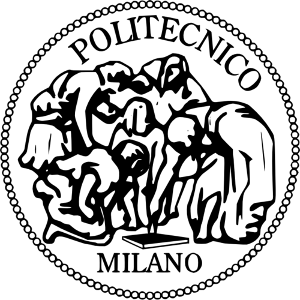
\includegraphics[width=0.3\textwidth]{Logo}
\end{figure}
\begin{center}
    \textsc{ \LARGE{Politecnico di Milano \\}}
	\textsc{ \Large {School of Industrial and Information Engineering\\ }}
	\vspace{3mm}
	\textnormal{ \Large{Software Engineering 2 Project\\}}
	\vspace{30mm}
	\fontsize{10mm}{7mm}\selectfont
    \textup{e-Mobility for All}\\
    \textnormal{ \LARGE{Design Document\\}}
\end{center}

\vspace{18mm}

\begin{center}
    \textnormal{\large{\bf Authors:\\}}
	{\large Enrico Brunetti \\ Matteo Gionfriddo }
	\fontsize{10mm}{5mm}\selectfont
\end{center}
\vspace{15mm}

\centering{\large{
Academic Year 2022/2023 \\
\vspace{10mm}
Milano, -/12/2022 \\
\vspace{2mm}
Version 1.0
}}

\end{titlepage}

\newgeometry{top=3cm}
\tableofcontents
\listoffigures
\begingroup
\let\clearpage\relax %avoid to put it on a new page
\listoftables
\endgroup
\restoregeometry

\chapter{Introduction}
\section{Purpose}

The purpose of this document is to detail the design of the software and of the architecture regarding the eMall system. The analysis has been made in a more detailed approach for the description of each component
and the overall architecture of the system, by also covering the relationships between each one of them. Furthermore has been inserted mockups of Mobile Application for End-Users and Web interface for CPOWs and a plan for the implementation,
testing and integration of the system.

\section{Scope}
\textit{eMall} is an application system designed for help End-Users to take advantage of the services for charging electric vehicles and helps Charging Point Operators manage associated charging
stations.\\
The End-Users can use the mobile app to browse a map that displays the charging stations nearby, their cost and any special offer they have and book and use an electric vehicle charge.\\
The CPO Workers can use the web application to manage their associated charging stations and interact with DSO in order to acquire energy furniture. The system is supported by APIs provided by a map service and suited for interaction between the various providers (eMSPs, CPOs, and DSOs) as explained in the RASD and in the following sections of this document.
\section{Definitions, Acronyms, Abbreviations}
\begin{itemize}
\item \textit{API}: Application Programming Interface.
\item \textit{DBMS}: Database Management System.
\item \textit{eMSP}: e-Mobility Service Provider.
\item \textit{CPO}: Charging Point Operator.
\item \textit{CPOW}: Charging Point Operator Worker.
\item \textit{CPMS}: Charge Point Management System.
\item \textit{DSO}: Distribution System Operator.
\end{itemize}
\section{Revision history}
\begin{itemize}
\item |-12-2022 Version 1.0.
\end{itemize}
\section{Reference Documents}
\begin{itemize}
\item Assignment Document "Assignment RDD AY 2022-2023\_v3.pdf"
\item RASD Document "RASD1.pdf"
\end{itemize}
\section{Document Structure}

The document consists of 7 different chapters:
\\
\\
\textbf{Chapter 1}: in this first chapter the purpose and the scope of this Design Document for eMall system are briefly presented. Furthermore, some basic information about acronyms and abbrevations is provided in order to help in the understanding of the whole document.\\ \\
\textbf{Chapter 2}: the second chapter purpose is to describe and motivate design choices. In particular, it starts with an overview of the chosen architecture from a more general and abstract perspective first to a more specific one consisting in the description of components then. After, interdependencies and interactions between different components are shown through different diagrams. In the end, also architectural styles, patterns and other minors design decisions are briefly reported. \\ \\
\textbf{Chapter 3}: here the two different types of user interfaces are presented. In particular, different mockups show how interfaces should be once implemented.\\ \\
\textbf{Chapter 4}: the fourth chapter contains all informations about requirement traceability. More specifically, it's described which requirements are satisfied by which components in a sort of mapping.\\ \\
\textbf{Chapter 5}: in this chapter, the testing implementation and integration for the system are described.\\ \\
\textbf{Chapter 6}: in this chapter, the effort spent by each team member is briefly presented in order to provide an overview of how the work has been done.\\ \\
\textbf{Chapter 7}: the last chapter contains the references used during the developing process of the document.

\chapter{Architectural Design}
\section{Overview:}
The architectural style chosen for the eMall system is a three-tiered architecture which exploits the client-server paradigm. Furthermore, the system can be divided into three different subsystems: the presentation layer, the application layer and the data layer. Each tier is responsible for one of the three layers. The first layer, the \textbf{Presentation} layer is made by the couple Mobile application-eMSP (that will be used by an End-User for doing actions such that view all prices and offers of nearby charging stations and/or booking and use an electric charge) and the Web application (that is destinated for a CPOW that needs to manage their associated charging stations and communicate with DSO in order to make energy furniture agreements) and provides the GUI of the system. The second layer, the \textbf{Logic} layer, implements all the logic of the application receiving and executing the requests done by the End-User or by the CPOW. The third layer, the \textbf{Data} layer stores and maintains all the data that the system needs in order to provide correctly the services offered by the system, such that all the users accounts, all bookings and all information about the charging stations registered.\\
The aim of the system architecture is to allow multiple eMSPs interact with multiple CPMS. Every eMSP is connected from one side to his associated Mobile Application in order to provide the Presentation layer, and from the other side communicates with the Logic layer. In this way, every End-User side GUI will have the same fundamental structure (that is optimized in order to communicate with the Logic layer of eMall), but will contain different design decisions that are different from one eMSP to another.
On the other hand the interaction with the CPMS is made by a proper CPMS API that is directly connected with the system. As can be seen clearly in the next section, the Logic layer of eMall can interact with a CPMS API in different ways, with the purpose to take into account every request that can be done by a CPOW.




\section{Component view}
The figure \ref{fig:general-component-diagram} is a \textit{Component Diagram} for the \textit{eMall} system that displays in an high level how every component are connected each other.

\begin{figure}[hp]
\centering
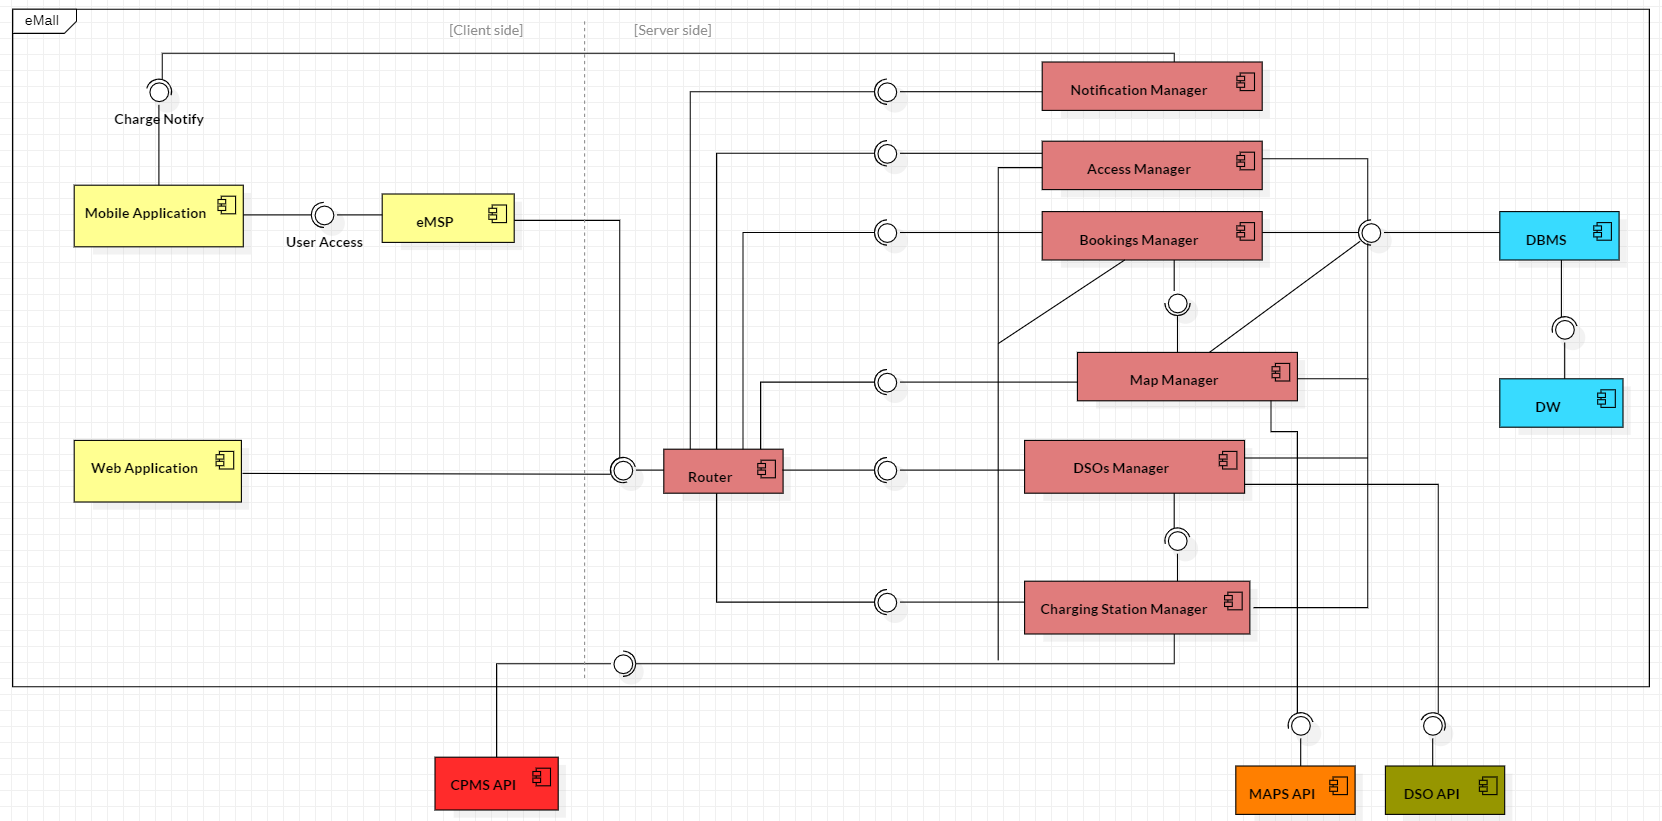
\includegraphics[scale=0.4 ]{img/GENERAL DIAGRAM_v2.png}
\caption{UML Component Diagram}
\label{fig:general-component-diagram}
\end{figure}


\begin{figure}[hp]
\centering
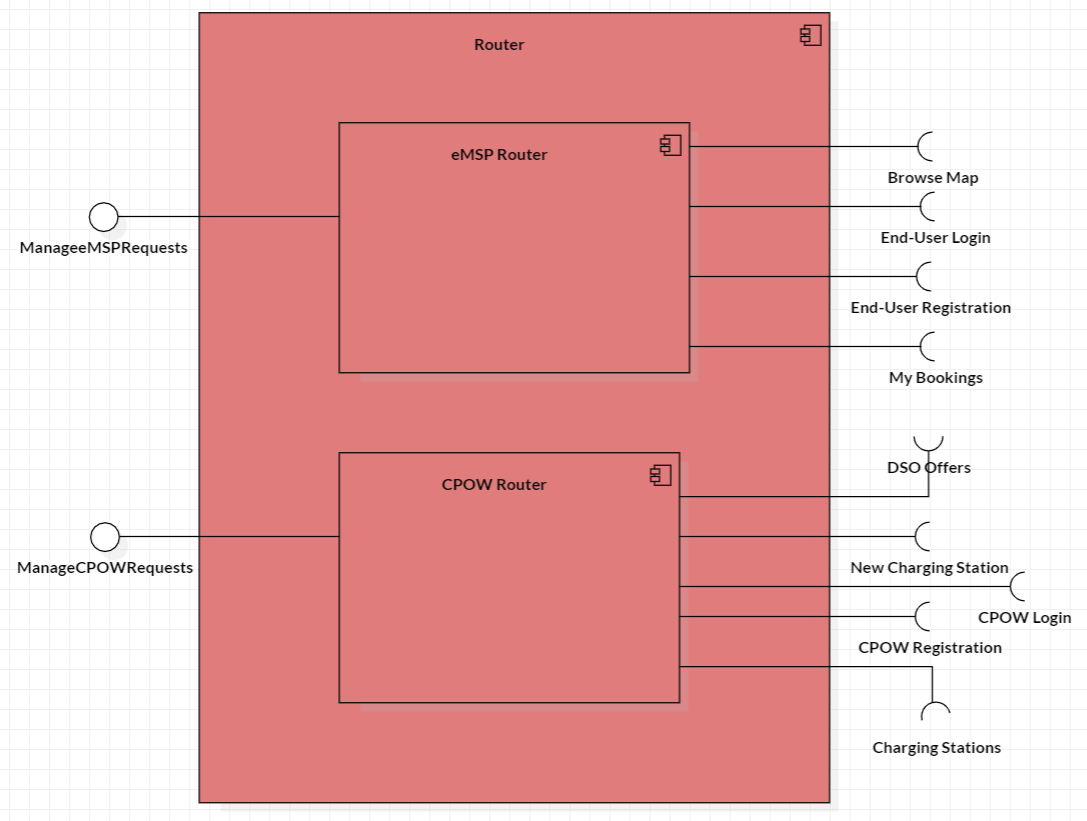
\includegraphics[scale=0.6]{img/ROUTER_v2.png}
\caption{UML Component Diagram for \textit{Router} component}
\label{fig:router-component}
\end{figure}

In this diagram when two components can communicate using different interfaces a single interface link is
reported, for the sake of readability. The various components are now described and detailed:
\begin{itemize}
\item \textbf{Router}: it dispatches the requests coming from the users applications. Figure \ref{fig:router-component} represent how is composed in detail.

\item \textbf{Bookings Manager}: it performs all operations related to the management of the charge bookings allowing to pick all personal bookings associated to an account and creating a new one,  interacting with the \textit{DBMS}. Moreover it allows to start a charging process talking directly with the \textit{CPMS API} and makes the End-User payment communicating with the \textit{Payment API}, in both cases via a dedicated interface. This component is described in figure \ref{fig:bookingsmgr-component} .


\begin{figure}[htp]
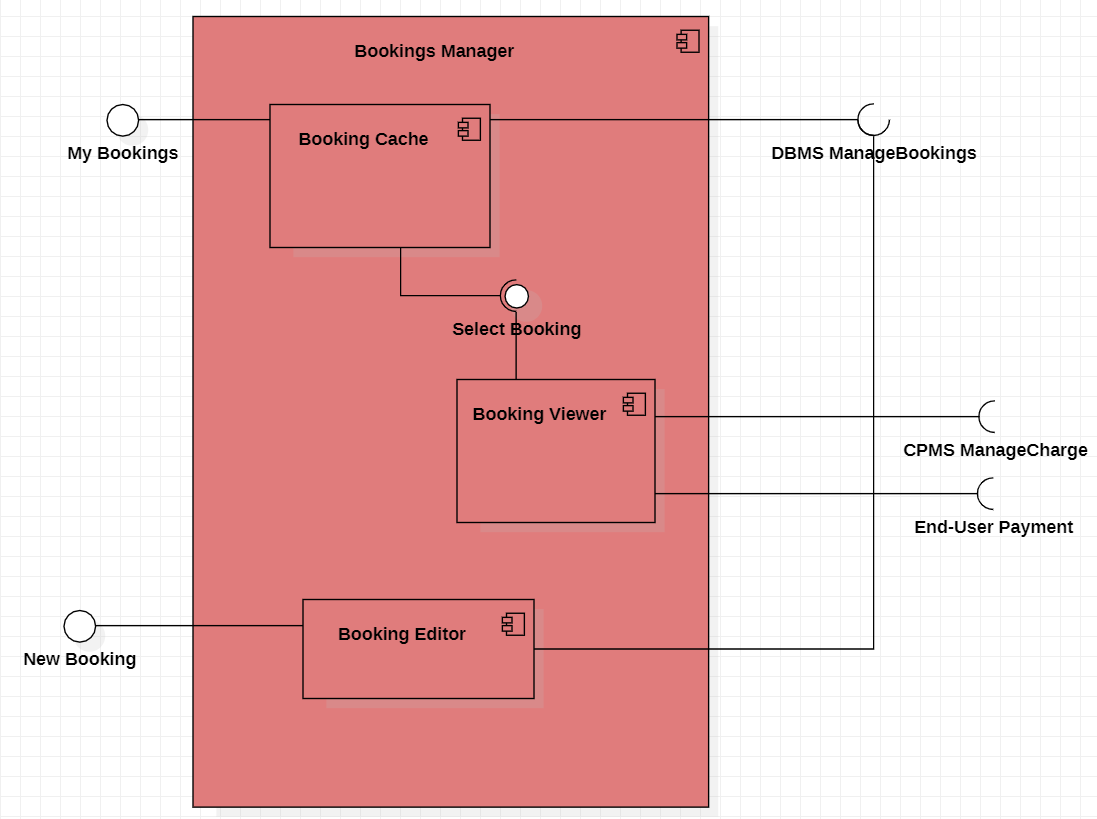
\includegraphics[scale=0.6]{img/BOOKINGS MANAGER.png}
\caption{UML Component Diagram for \textit{Bookings Manager} component}
\label{fig:bookingsmgr-component}
\end{figure}

\item \textbf{Access Manager}: it manages everything about registration and login of the users. It allows to create a new account and checks the login credentials communicating with the \textit{DBMS} and also checks if the data inserted during the registration is correct through interfaces connected with the \textit{Payment API}, \textit{Motorization API} and \textit{CMPS API}. This component is detailed in figure \ref{fig:accessmgr-component}.

\begin{figure}[htp]
\centering
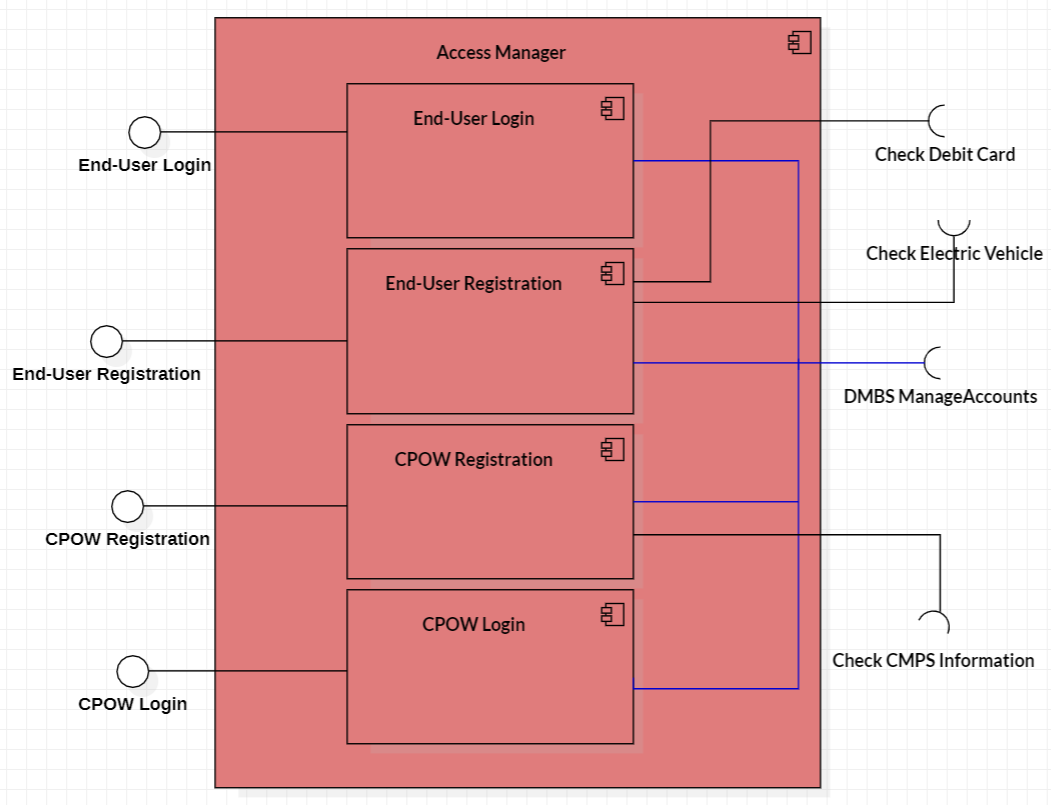
\includegraphics[scale=0.45]{img/ACCESS MANAGER.png}
\caption{UML Component Diagram for \textit{Access Manager} component}
\label{fig:accessmgr-component}
\end{figure}

\item \textbf{Charging Stations Manager}: it permits to view all charging stations associated to a certain CPMS and do all management operations for each one of them. It requires to communicate, by some interfaces, with the \textit{DBMS} component and the associated CPMS. If set properly, the sub-component \textit{Charging Station Viewer} can also interact automatically with the \textit{CPMS API}. It is shown in the diagram in figure \ref{fig:chargingstationsmgr-component}.


\begin{figure}[htp]
\centering
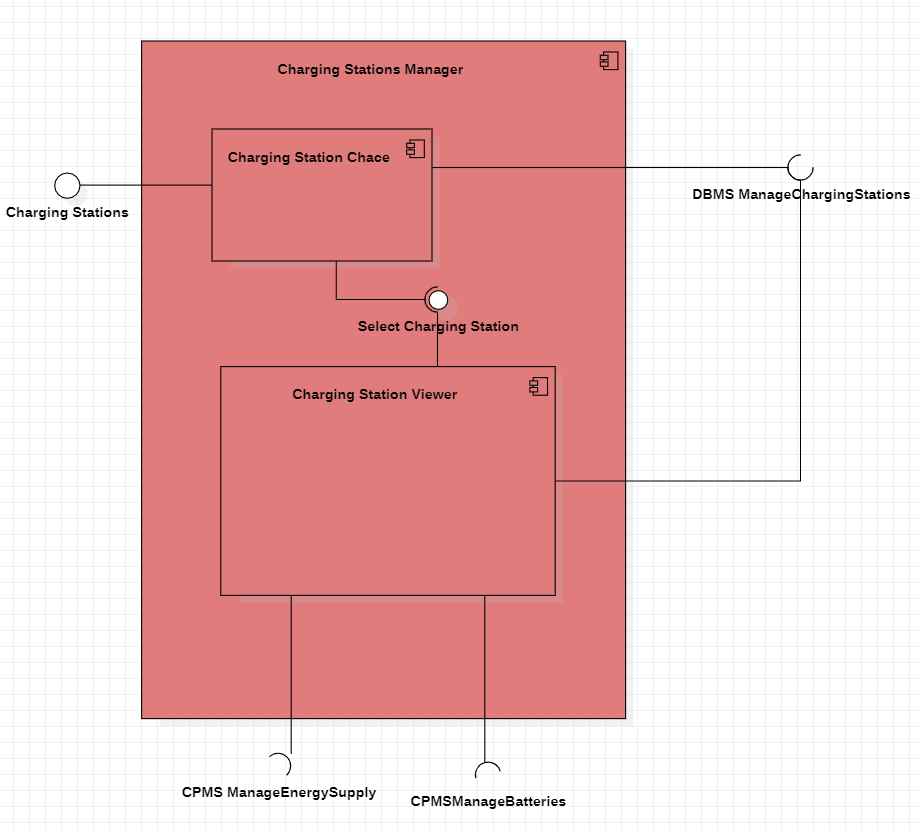
\includegraphics[scale=0.6]{img/CHARGING STATION MANAGER.png}
\caption{UML Component Diagram for \textit{Charging Stations Manager} component}
\label{fig:chargingstationsmgr-component}
\end{figure}

\item \textbf{Notification Manager}: it sends to the End-User the information about the state of a charging process. Indeed, it is connected to the \textit{CPMS API} and the \textit{Mobile Application} component via interfaces.

\item \textbf{Map Manager}: it builds the charging station map interacting with the \textit{DBMS} and with the \textit{Maps API}

\item \textbf{DSOs Manager}: it deals with everything about the management of DSO agreements. It is connected with the \textit{DSO API} in order to capture the DSOs offers and contact a DSO in order to make an energy furniture agreement and is also connected to the \textit{DBMS} with the purpose to get and save all DSO energy furniture of a certain CPMS.

\item \textbf{DBMS}: this component manages the operational database.

\item \textbf{Motorization API}: is an external component used to check the vehicle information inserted by an End-User.

\item \textbf{Payment API}: is an external component used to check the debit card information inserted by an End-User.

\item \textbf{Maps API}: is an external component used to retrieve maps for the realization of the charging stations map.

\item \textbf{CPMS API}: is an external component that permits to communicate with a CPMS.

\item \textbf{DSO API}: is an external component that allows to interact with a DSO.

\item \textbf{Mobile Application} and \textbf{eMSP}: they constitute together the \textit{Presentation Layer} for the mobile devices allowing the End-Users to use all services that the system offers, such that view nearby charging stations offers and book and use
electric vehicle charges,

\item \textbf{Web Application}: this component is the \textit{Presentation layer} of the web app which allows CPOW to interact with his associated CPMS in order to take management decision of the related charging stations.
\end{itemize}

Note : \textbf{Motorization API}, \textbf{Payment API} and \textbf{Maps API} are described in detail in the \textit{Components Interfaces} section.
\section{Deployment view}

A more detailed description of the system is given in this section. In figure \ref{fig:deployment-diagram} there is an UML Deployment Diagram which shows the allocation of the software components in the physical tiers of the system.

\begin{minipage}{\linewidth}
        \centering
        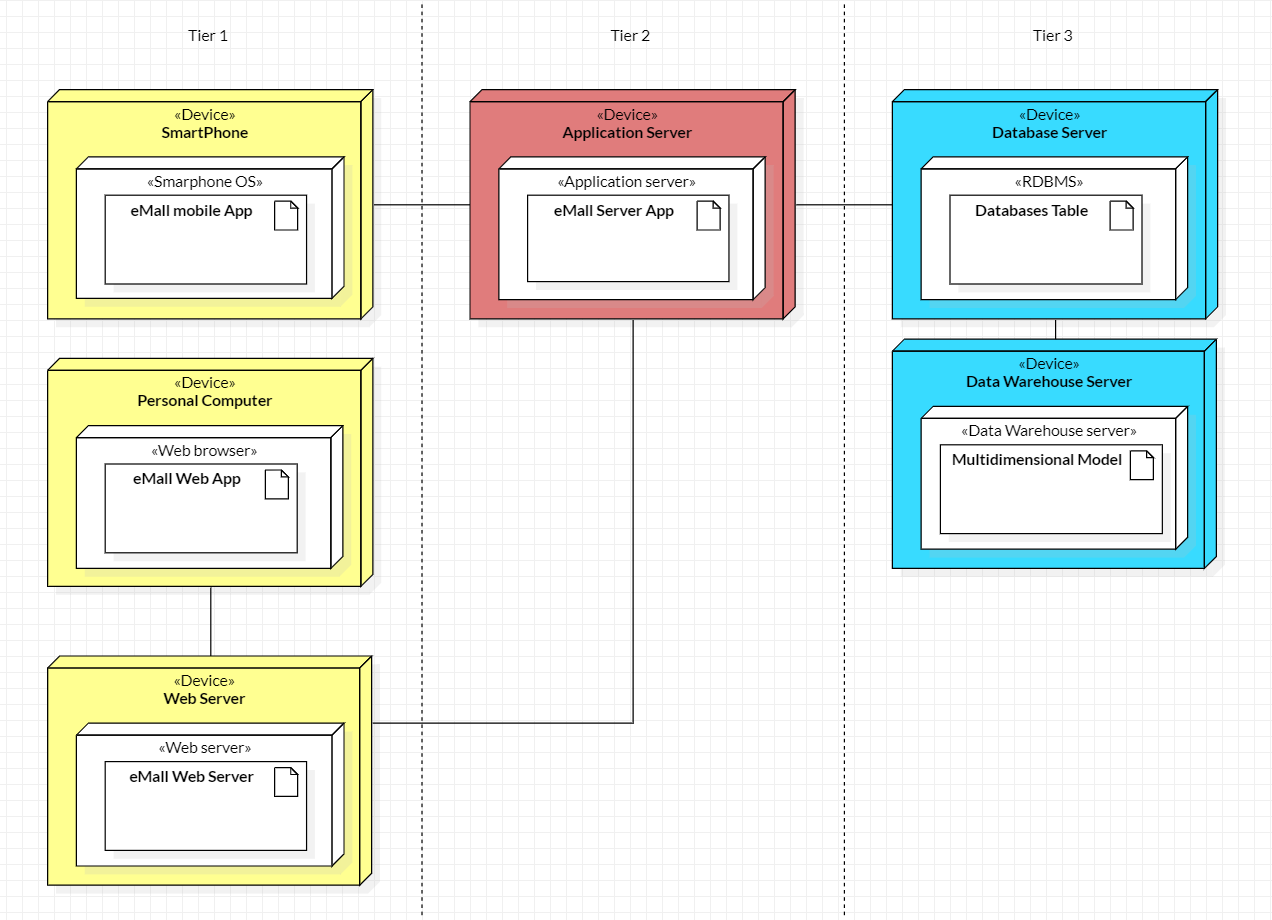
\includegraphics[scale=0.5]{img/DEPLOYMENT DIAGRAM.png}
        \captionof{figure}{UML Deployment Diagram}
        \label{fig:deployment-diagram}
\end{minipage}



$ $\newline
$ $\newline
As can be seen in the component diagram (figure \ref{fig:general-component-diagram}), the different colors indicate the allocation of components.
It's evident that about the first tier, the \textit{Smartphone} contains the mobile application while the \textit{Personal Computer} and the \textit{Web Server} contains the \textit{Web application}.\\
In the application logic all 'Manager' components are provided by the \textit{Application Server} while in the Data tier the \textit{DBMS} component is deployed by the \textit{Database Server}.\\
Is important to notice that from the Web side, the \textit{Presentation Layer} is contained by the \textit{Web App} that actually provides the graphic interface of the application, and by the \textit{WebServer} that however handle the client requests and responses interacting with the \textit{Application Layer}.


\section{Runtime view}

Figures \ref{fig:seq-registration}, \ref{fig:seq-login}, \ref{fig:seq-loadMap}, \ref{fig:seq-booking}, \ref{fig:seq-charge}, \ref{fig:seq-selectDSO}, \ref{fig:seq-energyManagement}, \ref{fig:seq-csStatus} are UML sequence diagrams exploited to show how the different components of the system interact each other during the execution of the most important functions provided. In order to show more cleaner and comprehensible diagrams, we assume that in all figures after \ref{fig:seq-login} users are already correctly logged in.
\\\\
In the sequence diagram of figure \ref{fig:seq-registration} the registration process of an End-User to the eMall system through the \textbf{Mobile Application} is shown. First of all the potential user must compile the registration form and, as a first check, the \textbf{Mobile Application} checks directly if provided data are in the correct format. Subsequently, an \textit{endUserRegistration} request is sent to the \textbf{eMSP} the user has decided to register to, which will send it to the \textbf{Router}, which will route it to the \textbf{Access Manager}. This component communicates with \textbf{Motorization API} in order to check if the driving license provided by the potential user exists and it's active. If all data are correct the \textbf{Access Manager} sends all of them to \textbf{DBMS} in order to store information about the new End-User and, in the end, a success message is shown on the \textbf{Mobile Application}. Also the registration process of a new CPOW works in the same way, exception for the fact that the CPMS identification has to be checked instead of the driving license. So, since the representation of that by a sequence diagram is very similar to this one and trivial, is not reported.
\\\\
In the sequence diagram of figure \ref{fig:seq-login} the End-User login process and the interactions between all components involved are shown in detail. First of all, an End-User must fill the respective form with username and password on \textbf{Mobile Application}. Inserted information reaches \textbf{Router} End-User's respective \textbf{eMSP}. Then the router will route them to \textbf{Access Manager}, which will ask the \textbf{DBMS} to provide the stored password related to that specific user. Subsequently, the \textbf{Access Manager} checks if the password provided by \textbf{Mobile Application} is equal to the one provided by the \textbf{DBMS}. If it's not the case a login error is sent back to the \textbf{Mobile Application}, which allows the user to retry again inserting the correct data. On the other hand, if the data were correct, the user is successfully logged in, a new token associated with the specific logged user is generated and stored in the \textbf{DBMS} and, in the end, the End-User is notified of login success. Also in that case, the sequence diagram of CPOW login is not provided since it works exactly in the same way.
\\\\
In the sequence diagram of figure \ref{fig:seq-loadMap} the functionality which allows the \textbf{Mobile Application} to show a map of all available charging stations is shown. Note: this function can take place independently from the fact that the End User is logged in or not since all available charging stations are shown also to not registered users. In detail GPS coordinates of End-User are routed from the \textbf{Router} to the \textbf{Map Manager} that will get an updated world map from \textbf{MAPS API}. Then, the \textbf{Map Manager} gets from the \textbf{DBMS} all information about charging stations in a certain range of distance from provided coordinates and mounts charging stations on the map, exploiting their coordinates. After, the updated map will be returned to \textbf{Mobile Application} that will load it and show it to End-User.
\\\\
In the sequence diagram of figure \ref{fig:seq-booking} the whole charge booking process is presented together with relations between all involved components. First of all, a logged-in End-User must select a charging station, a socket type, and a date from the \textbf{Mobile Application}. After that, the router will receive a get availability request from the involved \textbf{eMSP} and will route it to \textbf{Booking Manager}, that will get from \textbf{DBMS} all availability for that specific day. If there is at least one are all sent to \textbf{Mobile Application}, otherwise, an error is sent back. At this point, the End-User must select, through the \textbf{Mobile Application}, a time slot from the available ones, a vehicle, and also a payment method from the ones connected to his account. A booking request will after follow the same path as before in order to reach the \textbf{Booking Manager}, which will exploit the \textbf{Payment API} in order to check if the selected payment method has enough funds for the payment and provisionally block them. If that operation has success the new booking is stored in the \textbf{DBMS} and a success message is sent back to the \textbf{Mobile Application}, otherwise, a booking error is returned.
\\\\
In the sequence diagram of figure \ref{fig:seq-charge} is presented how all components react and interact with each other during a whole charging process that is assumed to have been already booked. First of all, a correctly logged-in End-User, which is assumed to be near the right charging column, must click on the start charging button of the \textbf{Mobile Application}, which will send the request with the associated \textit{id} to the \textbf{Router}, trough the \textbf{eMSP}. Then, the request is routed to the \textbf{Booking Manager} that will ask all dates about the specific charge to the \textbf{DBMS} and then will check them. If the charge exists and it's the right time, the \textbf{Booking Manager} sends, through the \textbf{Router}, an \textit{abilitateCharge} message to the \textbf{Charging Station Manager} for that specific charge at that specific time in that specific socket of that specific charging station. After that, the \textbf{Booking Manager} sends also a \textit{charge\_can\_start} message to the mobile application. At this point, the user approaches his mobile phone to the RFID reader of the charging socket and the \textbf{Charging Station API} sends a get enabling message to the \textbf{Charging Station Manager} for the specific charge \textit{id} obtained through RFID. If the \textit{id} is correct the charge starts and the \textbf{Charging Station API} sends periodically to the \textbf{Charging Station Manager} the current status of recharge, which will be reported, firstly to the \textbf{DBMS} and secondly, through the \textbf{Router}, as a \textit{current\_status} messages to the \textbf{Mobile Application} that displays charging status to the End-User. When the charge is completed, the \textbf{Charging Station API} communicates it to the \textbf{Charging Station Manager} that will save it to the \textbf{DBMS} and then ask, always through the \textbf{Router}, to the \textbf{Notification Manager} to send a notification of completed charge directly to the \textbf{Mobile Application}, that will show it to the user that will consequently remove the plug. To keep this heavy diagram a little cleaner has not been represented the fact that when the charge is complete, funds are charged to the End-User payment method from \textbf{Payment API}, and also this information is stored in the \textbf{DBMS}.
\\\\
In the sequence diagram of figure \ref{fig:seq-selectDSO} is presented the process of DSO selection from the CPOW point of view by showing how different involved components communicate with each other. First of all, an already logged-in CPOW must ask from the \textbf{Web Application} for all available DSOs for a specific charging station (this depends on the charging station location, i.e. different geographical areas may have different DSOs). Then a get DSOs request will follow the following path: \textbf{Web Application}-\textbf{Router}-\textbf{DSO Manager}. This last component will after get from \textbf{DSO API} the updated list of all available DSOs, check which ones are available for the specific charging station (after getting charging station data from \textbf{DBMS}), and then finally return back a list that is shown by the \textbf{Web Application}. At this point, the CPOW, through his web interface, selects one DSO and a change DSO request travels until reaches \textbf{Charging Station Manager}, that checks if the selected DSO is already active for that specific charging station. If it's not the case, a change DSO request is sent firstly to the \textbf{DSO Manager} that will communicate to \textbf{DSO API} the change and secondly another request is sent to \textbf{CPMS API}, in order to apply the effective changing to the charging station. At the end, the new DSO status for the charging station is stored from the \textbf{Charging Station Manager} to the \textbf{DBMS} and a success message is sent back to the \textbf{Web Application}. On the other hand, if the DSO is already selected for that specific charging station the system returns a message, and nothing changes.
\\\\
In the sequence diagram of figure \ref{fig:seq-energyManagement} is shown the process through which a CPOW can perform operations of charging station management exploiting the \textbf{Web Application}. In this particular example, we describe how that works in the case of enabling battery usage, but we can assume that the process is quite the same for all other similar operations, e.g. disabling batteries. First of all, an use batteries request for a specific charging station is routed by the \textbf{Router} from the \textbf{Web Application} to the \textbf{Charging Station Manager}. Then, this last component gets the current energy usage status of the selected charging station from the \textbf{DBMS} and checks if batteries are already enabled for that charging station. If it is the case an \textit{already\_using\_batteries} message is sent back to the \textbf{Web Application} and nothing changes. If it is not, the \textbf{Charging Station Manager} communicates to the \textbf{CPMS API} to enable batteries and update the charging station status on the \textbf{DBMS}. In the end, a success message is sent back to the \textbf{Web Application}.
\\\\
In the sequence diagram of figure \ref{fig:seq-csStatus} the focus is on how the \textbf{Web Application} gets all data about charging stations and is able to show them to a CPOW. When a CPOW opens his web interface connecting to the \textbf{Web Application} a request to obtain a list of all charging stations of his CPO passes through the \textbf{Router} and reaches the \textbf{Charging Station Manager}, which will get the list from the \textbf{DBMS} and return it back to the \textbf{Web Application} following the same path. At this point, when the CPOW selects a specific charging station on which to see all details and information, another get info request will follow again the path, but this time it's specific to a charging station. When this request reaches the \textbf{DBMS} it starts to send back, again on the path, all data to the  \textbf{Web Application} every 5 seconds, to ensure that data are always updated (e.g. if another CPOW or the system dynamically has disabled batteries). This loop ends when the CPOW exit the page of that specific charging station on the web interface of the \textbf{Web Application} and then the \textbf{DBMS} is informed to stop sending data.

\begin{landscape}
\begin{figure}[hp]
\centering
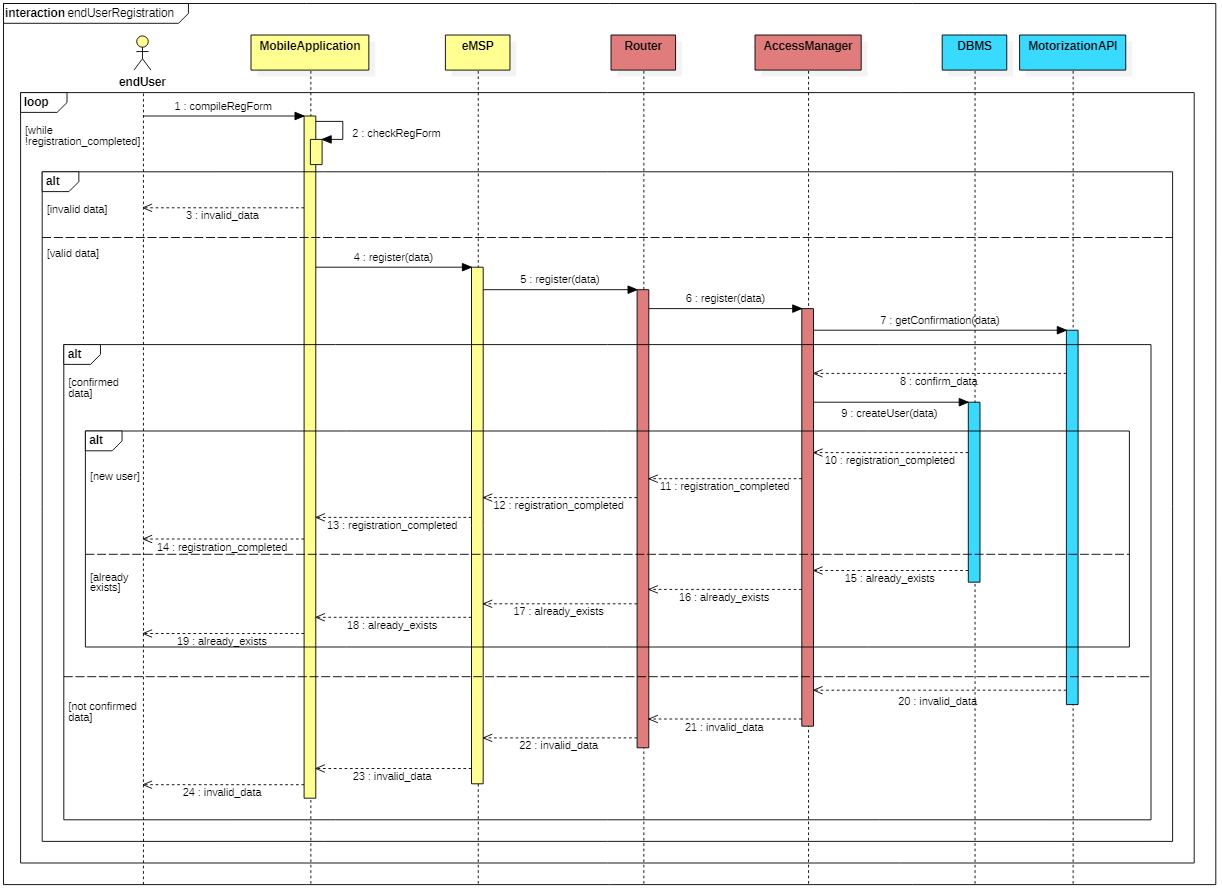
\includegraphics[scale=0.6]{img/sequenceRegistration.png}
\caption{UML Sequence Diagram for the End-User Mobile App registration}
\label{fig:seq-registration}
\end{figure}
\end{landscape}

\begin{landscape}
\begin{figure}[hp]
\centering
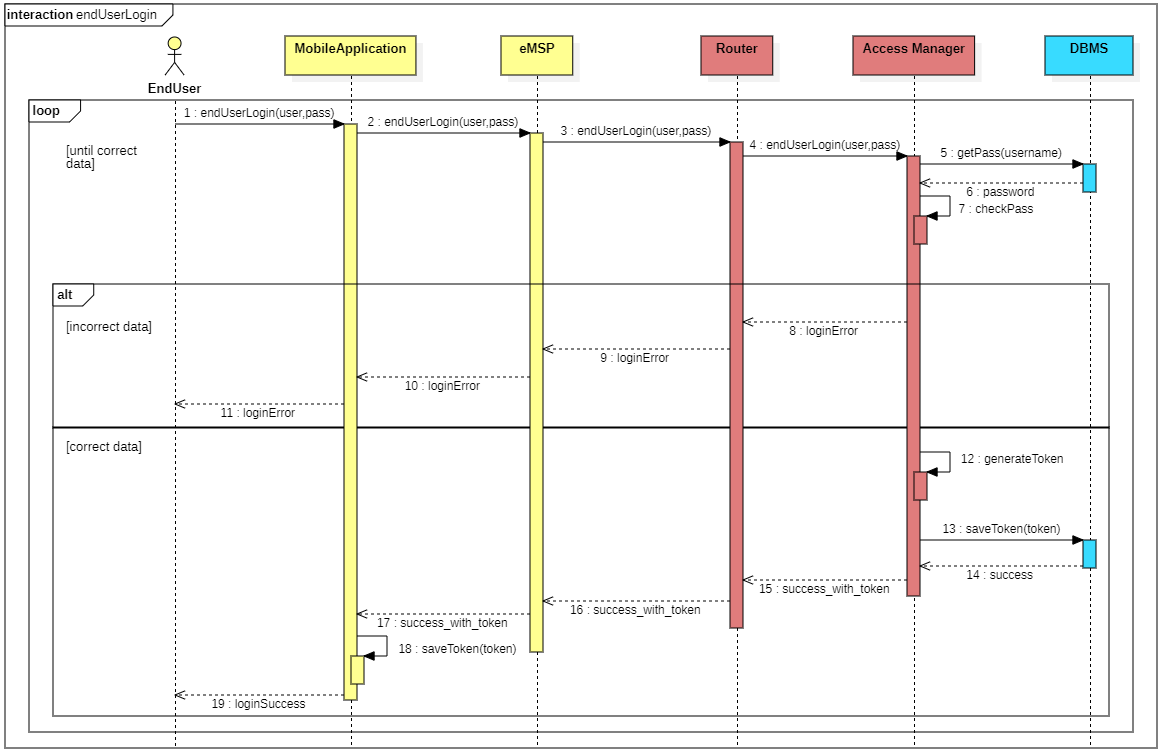
\includegraphics[scale=0.6]{img/sequenceLogin.png}
\caption{UML Sequence Diagram for the End-User Mobile App login}
\label{fig:seq-login}
\end{figure}
\end{landscape}

\begin{landscape}
\begin{figure}[hp]
\centering
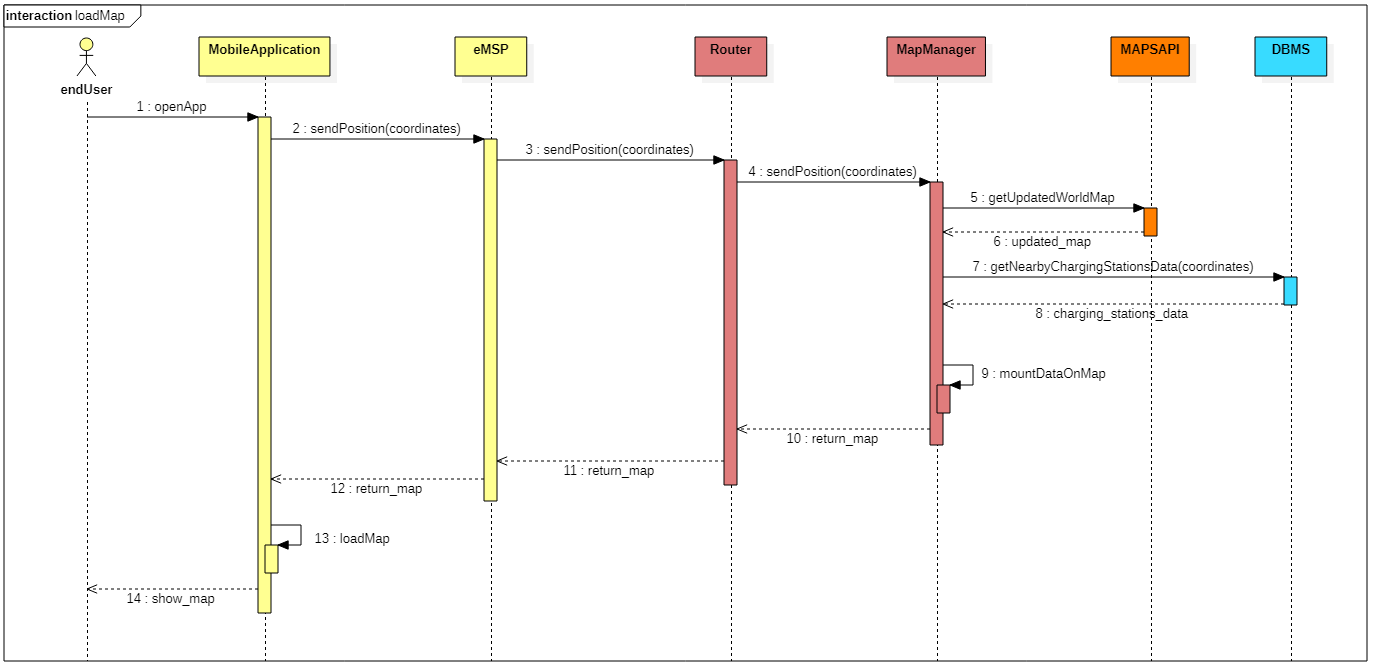
\includegraphics[scale=0.6]{img/sequenceLoadMap.png}
\caption{UML Sequence Diagram for Mobile App map load}
\label{fig:seq-loadMap}
\end{figure}
\end{landscape}

\begin{landscape}
\begin{figure}[hp]
\centering
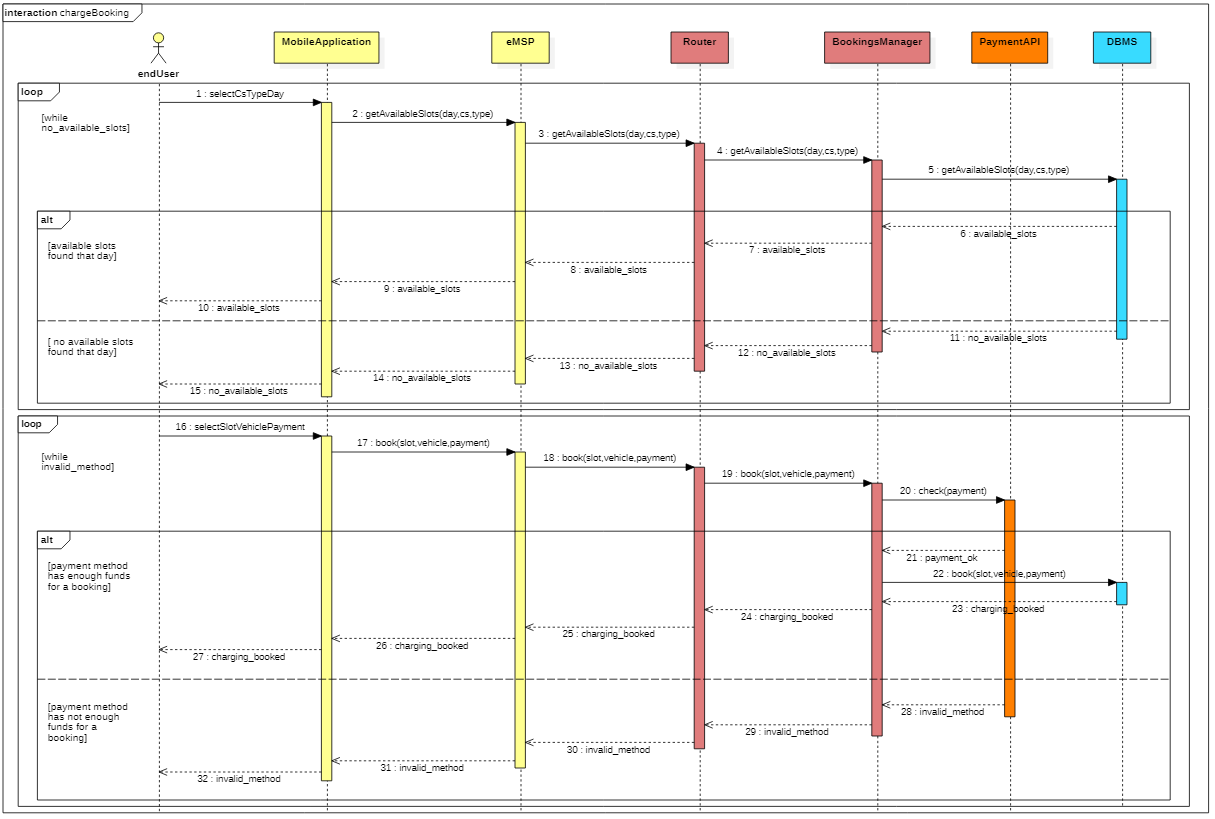
\includegraphics[scale=0.6]{img/sequenceChargeBooking.png}
\caption{UML Sequence Diagram for End-User charge booking}
\label{fig:seq-booking}
\end{figure}
\end{landscape}

\begin{landscape}
\begin{figure}[hp]
\centering
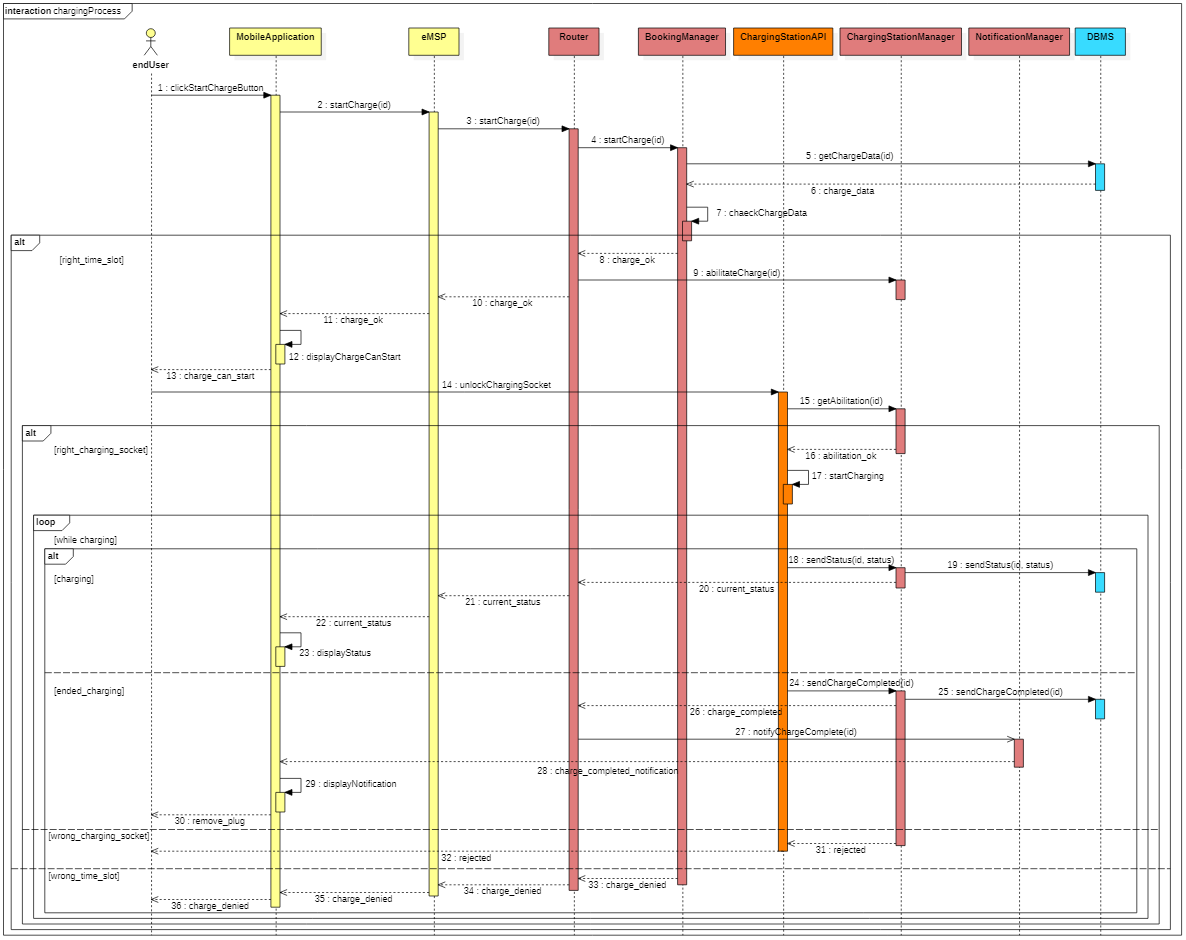
\includegraphics[scale=0.6]{img/sequenceChargingProcess.png}
\caption{UML Sequence Diagram for End-User charging process}
\label{fig:seq-charge}
\end{figure}
\end{landscape}

\begin{landscape}
\begin{figure}[hp]
\centering
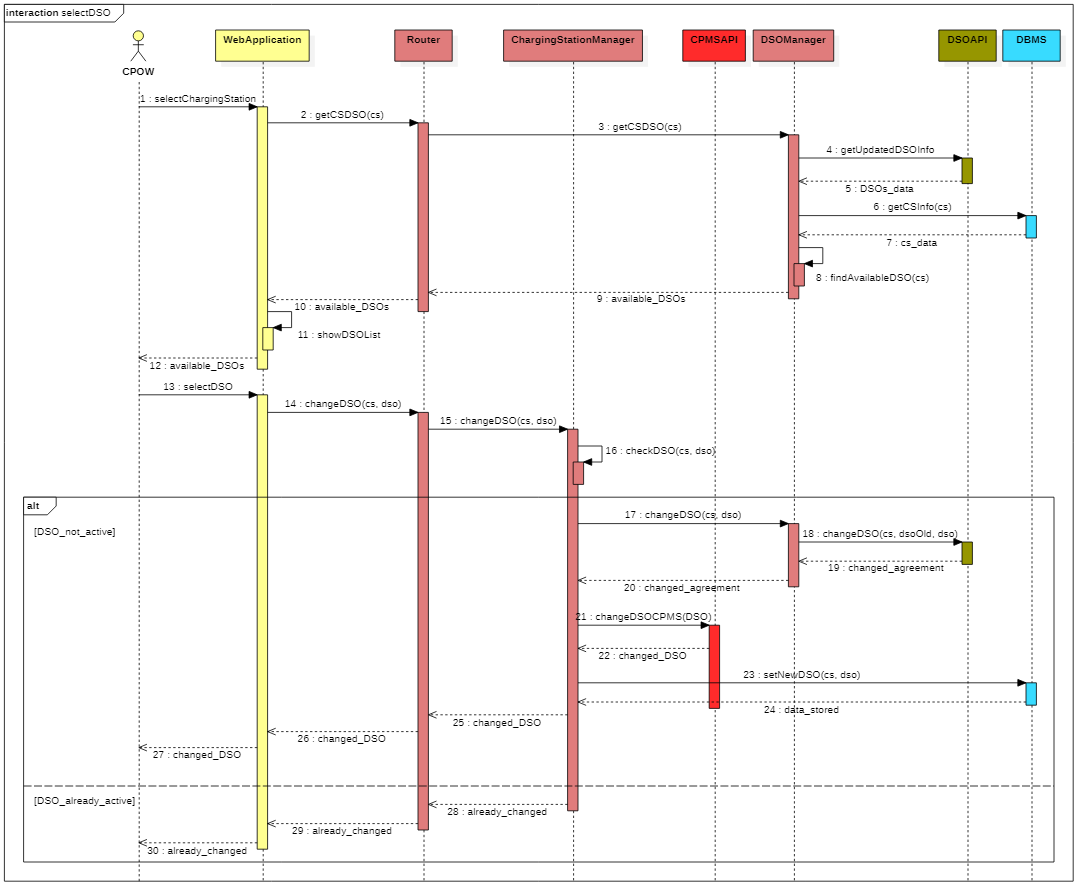
\includegraphics[scale=0.6]{img/sequenceSelectDSO.png}
\caption{UML Sequence Diagram for CPOW selecting a DSO for a charging station}
\label{fig:seq-selectDSO}
\end{figure}
\end{landscape}

\begin{landscape}
\begin{figure}[hp]
\centering
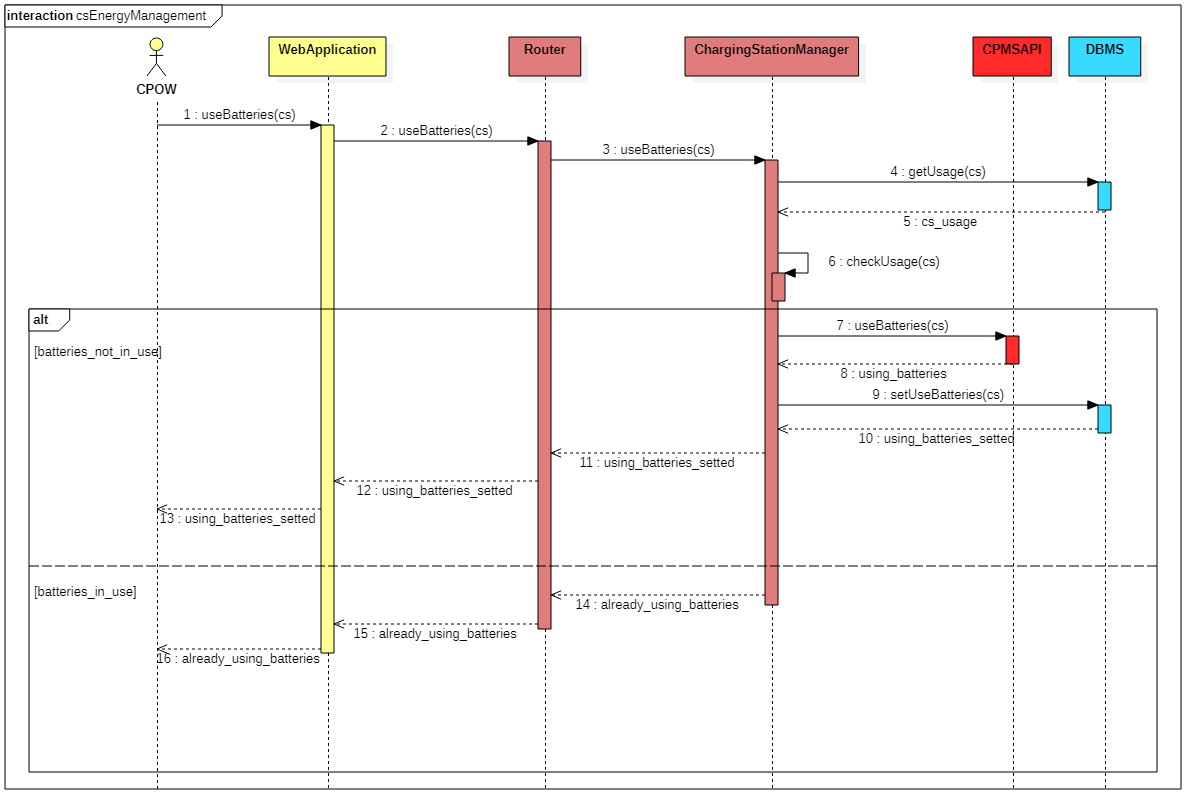
\includegraphics[scale=0.6]{img/sequenceCsEnergyManagement.png}
\caption{UML Sequence Diagram for CPOW selecting batteries usage for a charging station}
\label{fig:seq-energyManagement}
\end{figure}
\end{landscape}

\begin{landscape}
\begin{figure}[hp]
\centering
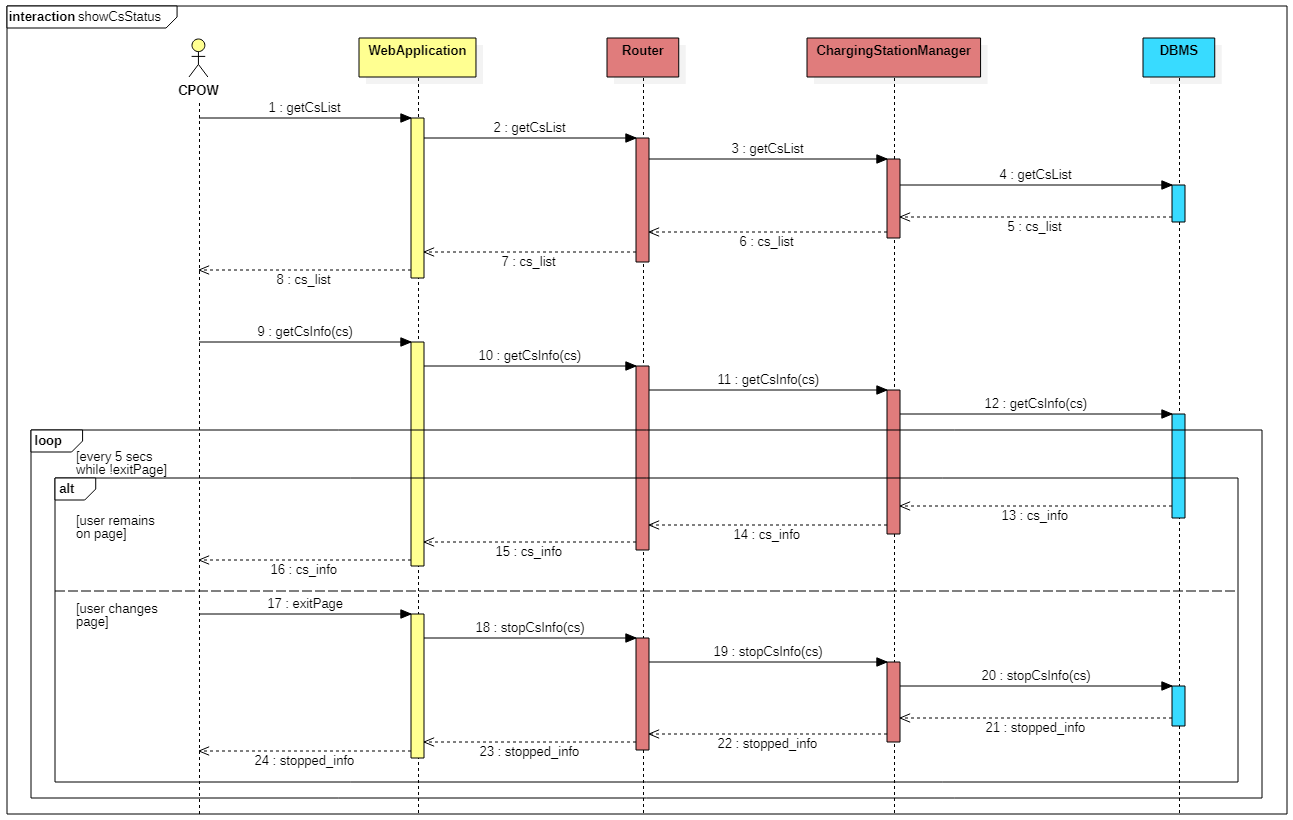
\includegraphics[scale=0.6]{img/sequenceShowCsStatus.png}
\caption{UML Sequence Diagram for Web Application showing to a CPOW date about a charging station}
\label{fig:seq-csStatus}
\end{figure}
\end{landscape}

\section{Component Interfaces}
In the diagram of figure \ref{fig:componentInterfaces} all component interfaces are described with respect to what is shown in the component diagram of figure \ref{fig:general-component-diagram}.

\begin{figure}[htp]
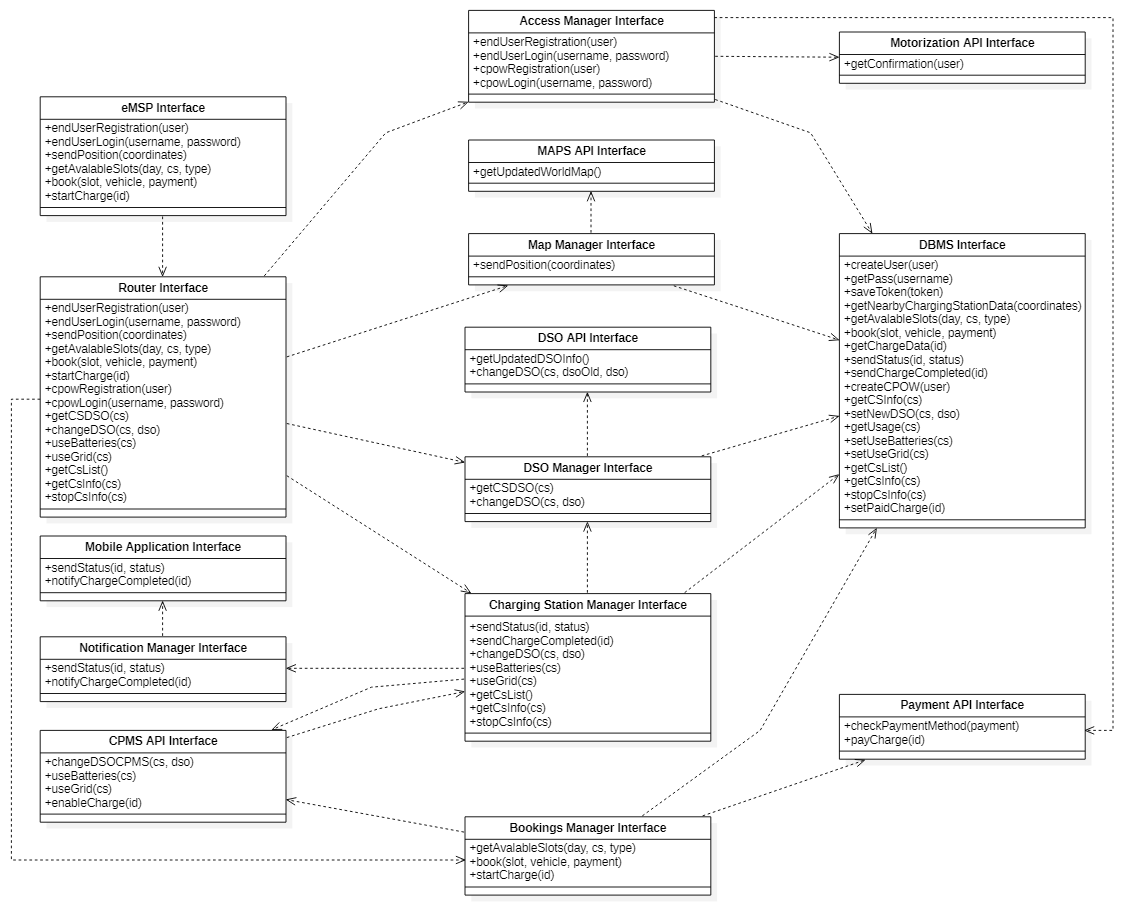
\includegraphics[scale=0.55]{img/componentInterfaces.png}
\caption{UML Interfaces Diagram}
\label{fig:componentInterfaces}
\end{figure}

In figure \ref{fig:classDiagram} is reported the Class Diagram already provided in the RASD document with a modification. During the develop of Design Document, considering all system requirements and functions to be implemented would have been useless to maintain a ChargingColumn class which has been removed with respect to the RASD version of the diagram. Charging columns numbers are now described as attributes of ChargingSocket class since their only usage could be for descriptive purpose. The diagram is still high level and it could be more refined before the effective implementation.

\newgeometry{top=0.1cm}
\begin{figure}[htp]
\includegraphics[width=\textwidth]{img/classDiagramDD.png}
\caption{UML Class Diagram}
\label{fig:classDiagram}
\end{figure}
\restoregeometry

\section{Selected architectural styles and patterns}

\subsection{Model-View-Controller Pattern (MVC)}
The eMall system is built exploiting the Model-View-Controller pattern in order to achieve some important benefits like:
\begin{itemize}
    \item Easier building of large-scale applications.
    \item Easily Modifiable: allows easy modification of the entire application and helps to increase flexibility and scalability.
    \item Faster development process: As there is segregation of the code among the three levels, developing web applications using the MVC pattern allows one developer to work on a particular section (say, the view) while another can work on any other section (say, the controller) simultaneously. This allows for easy implementation of business logic as well as helps to accelerate the development process.
    \item Easy planning and maintenance: MVC pattern is also helpful during the initial planning phase of the application because it gives the developer an outline of how to arrange their ideas into actual code. It is also a great tool to help limit code duplication, and consequently, allow easy maintenance of the application.
    \item Multiple views: following the MVC pattern, it's also easy to develop more view components for model components limiting code duplication as it separates data and business logic. This was particularly useful for eMSP and Web Application view components.
\end{itemize}
In the component diagrams of figure \ref{fig:general-component-diagram} and also in other diagrams like the sequence ones, different colors have been used to underline the different tiers of the pattern and their different functionalities. In particular, yellow components are view components, red components are controller components and blue components are model ones.

\subsection{Tiny client}
The eMall system is developed on a three-tier architecture, as previously explained. Furthermore, the client is thin, which means that, in this specific case, the client doesn't need to make particular computations or know anything about the system logic but has only a presentation purpose to the final user. This implies hardware resource optimization, reduced software maintenance, and improved security and in particular, is meaningful for both Mobile Application and Web Application.

\subsection{RESTful architecture}
The eMall system has been developed following also the REST architecture. The main motivations are:
\begin{itemize}
    \item RESTful system can be used by any type of client, regardless of programming language or execution environment.
    \item REST uses a stateless approach, which means that request state information is provided by the client to the server, allowing for greater scalability compared to other architectures that require server-side storage of state information.
    \item REST is based on the HTTP standard, which makes it easily interoperable with other technologies based on HTTP, such as our Web Interface.
    \item REST uses a cache-based approach, which can improve system performance as responses can be easily cached and reused in the event of future requests.
    \item REST uses a simple interface based on URI and HTTP verbs, which makes it easy to understand and use.
\end{itemize}

\subsection{Database}
The final database choice for eMall is a relational one since all data have pretty well-defined structures. We have a lot of entities (e.g. user, vehicle, booking, charging station, cpow, etc.) whose instances have been easily stored in relational tables that are accessed by SQL queries.

\section{Other design decisions}

\subsection{Maps API}
Since for this system is not worthy to develop, maintain and update a dedicated map system the final decision is to rely on an external service represented by the MAPS API Component. In particular, we will exploit google maps APIs, since are well documented, easy to implement and with a lot of features that allow to add markers and signals that represent the different charging stations directly on the map that is in the end sent to the Mobile Application.

\subsection{Motorization API}
Another necessity of the system is to check if the driving licences provided by users are vaild, in other words if users are enabled to drive the vehicle they want to book a charge for. This is made by the Motorization API component which exploits, for italian driving licences, the APIs, provided after have received an authorization, from the government website of ministry of infrastructure and transport. For driving licences of all other countries is assumed to obtain the same data from respective government websites.

\subsection{Payment API}
Also for the payment processing and for checking if the amount available on end user debit or credit cart is enough isn't worthy to develop a proprietary system. The final decision is to exploit a third party service, called Stripe, that supports a wide range of payment types, including major credit and debit cards, Apple Pay, Google Pay, and other digital wallets. It provides also an advanced fraud protection and compliance features to help ensure the security of transactions. Furthermore has a good documentation and a customer service that can help in setting up this side of the system.

\chapter{User interface design}
In this chapter are presented mobile application and web application mockups.

\begin{figure}[hp]
\centering
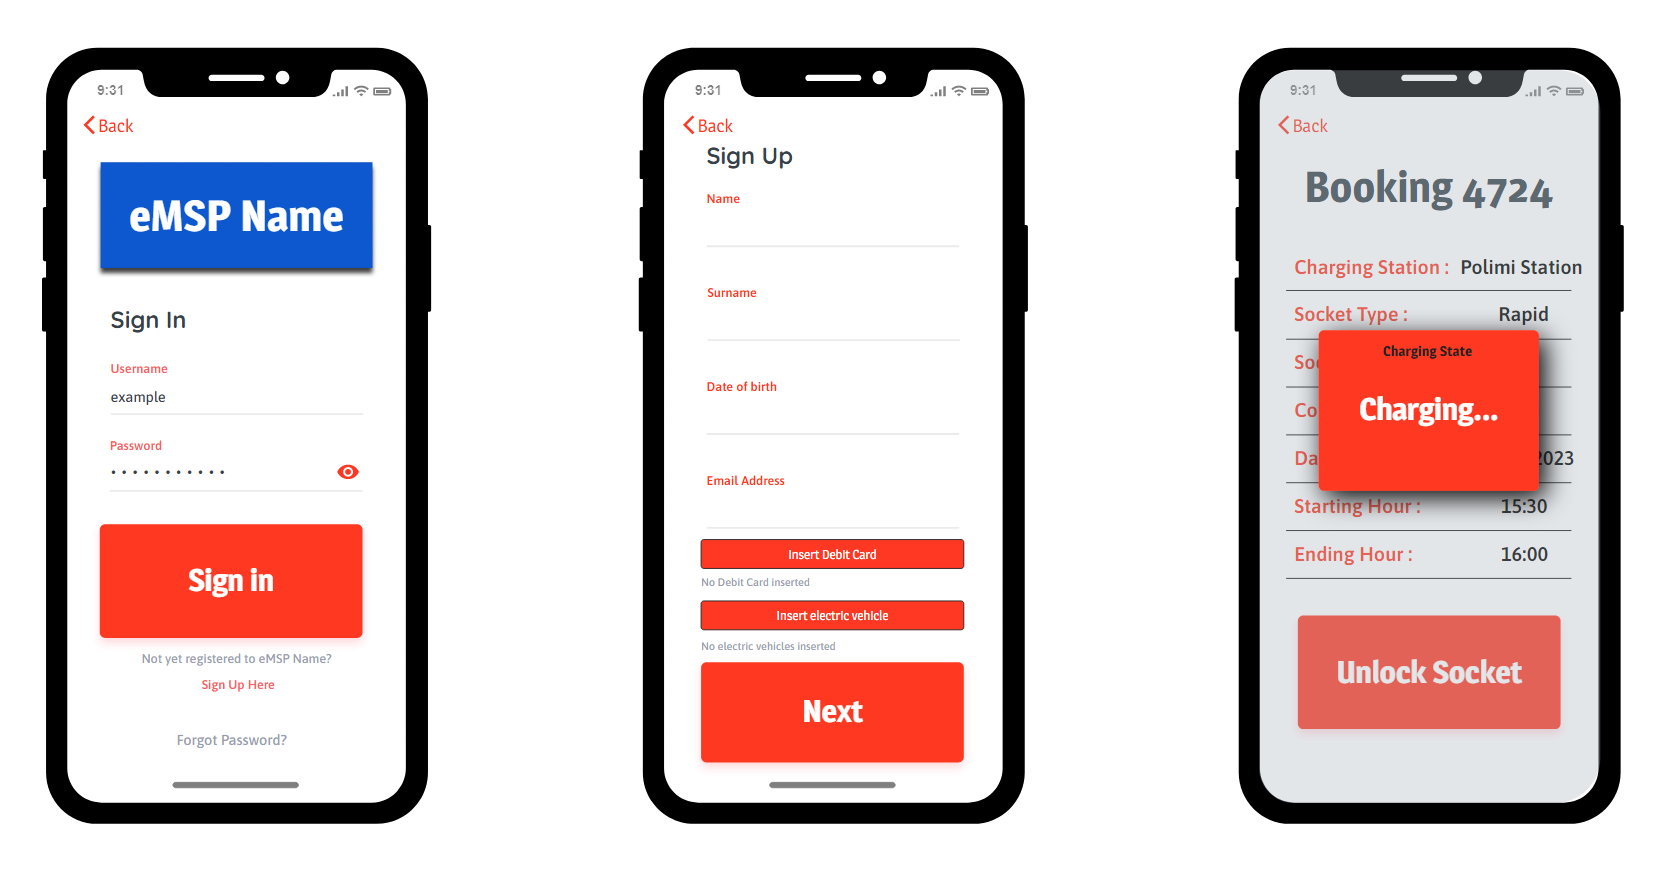
\includegraphics[scale=0.45]{img/mockups/MCKP1.png}
\caption{Mobile Application Mockups for End-User Log in, End-User Registration and Vehicle Charging State Popup Screens}
\label{fig:MobileApp-activity}
\end{figure}

\begin{figure}[hp]
\centering
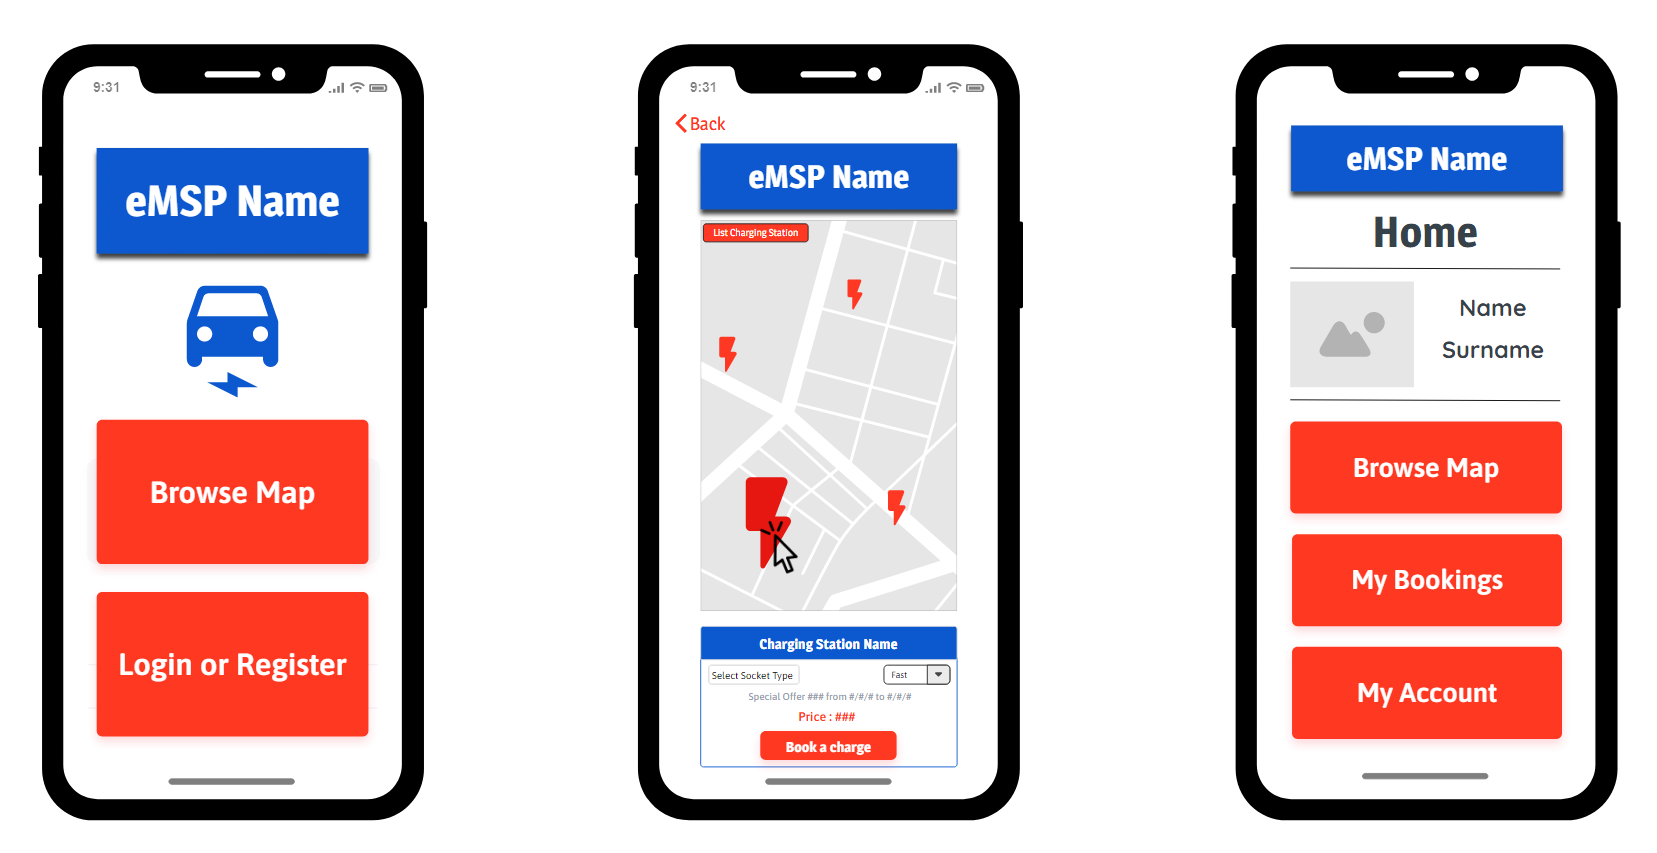
\includegraphics[scale=0.45]{img/mockups/MCKP2.png}
\caption{Mobile Application Mockups for Home Page, Charging Stations Map and Personal Home Page Screens}
\label{fig:MobileApp-activity}
\end{figure}

\begin{figure}[hp]
\centering
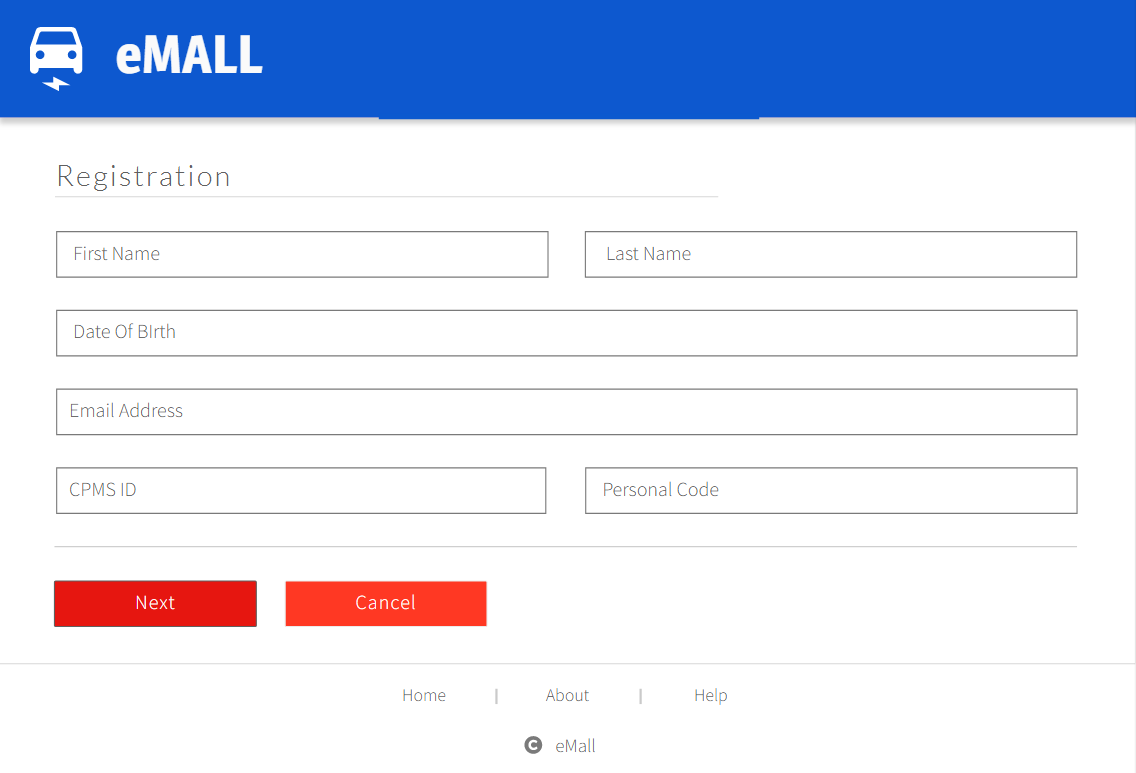
\includegraphics[scale=0.6]{img/mockups/MCKP_CPOWRegistration.png}
\caption{Web Application Mockup for CPOW Registration Screen}
\label{fig:MobileApp-activity}
\end{figure}


\begin{figure}[hp]
\centering
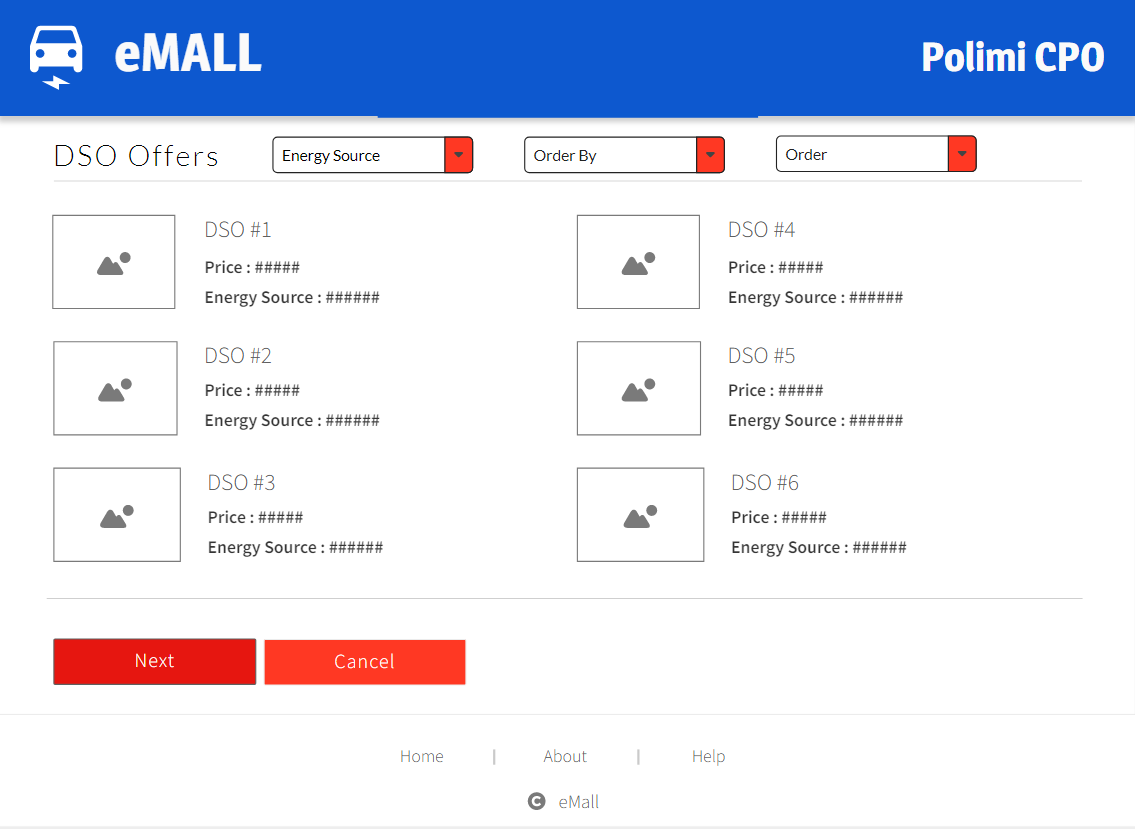
\includegraphics[scale=0.6]{img/mockups/MCKP_DSOoffers.png}
\caption{Web Application Mockup for DSO Offers Screen}
\label{fig:MobileApp-activity}
\end{figure}


\begin{figure}[hp]
\centering
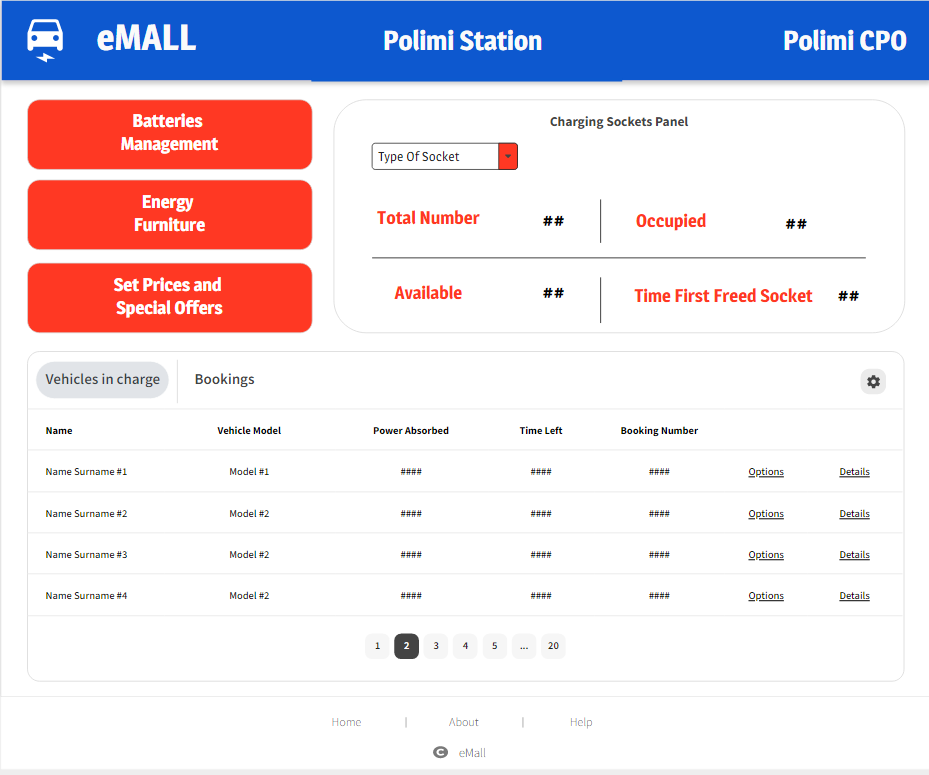
\includegraphics[scale=0.6]{img/mockups/MCKP_SelectedChargingStation.png}
\caption{Web Application Mockup for Selected Charging Station Screen}
\label{fig:MobileApp-activity}
\end{figure}

In the figures \ref{fig:MobileApp-activity}, \ref{fig:SupWebApp-activity}  are shown activity diagrams that describe how a End-User can navigate in the UIs offered by the application. Notice that  End-Users can quit the application from any state to reach the end state of the diagrams. No end state is represented and so are all the arrows that lead to them; this has been done for the sake of readability of the diagrams.

\afterpage{
\begin{landscape}
\begin{figure}[hp]
\centering
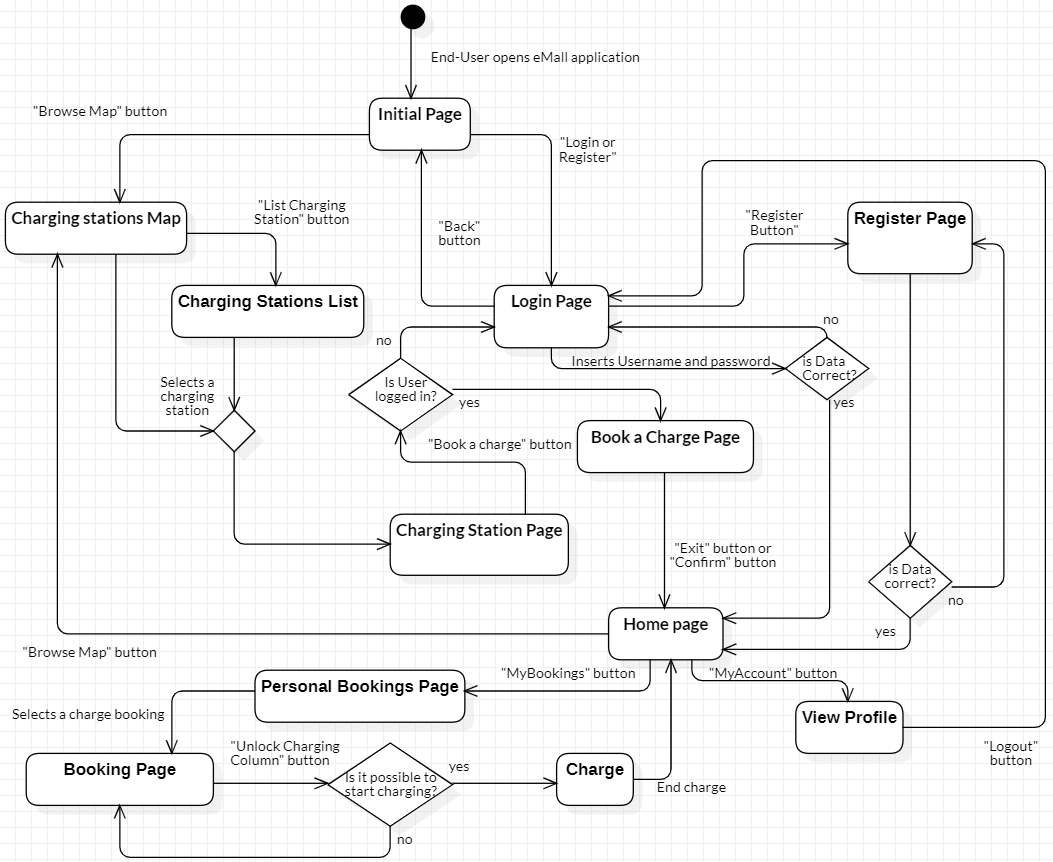
\includegraphics[scale=0.9]{img/ACTIVITY DIAGRAM END-USER.png}
\caption{UML Activity Diagram for the End-User Mobile App navigation}
\label{fig:MobileApp-activity}
\end{figure}
\end{landscape}

\begin{landscape}
\centering
\begin{figure}[hp]
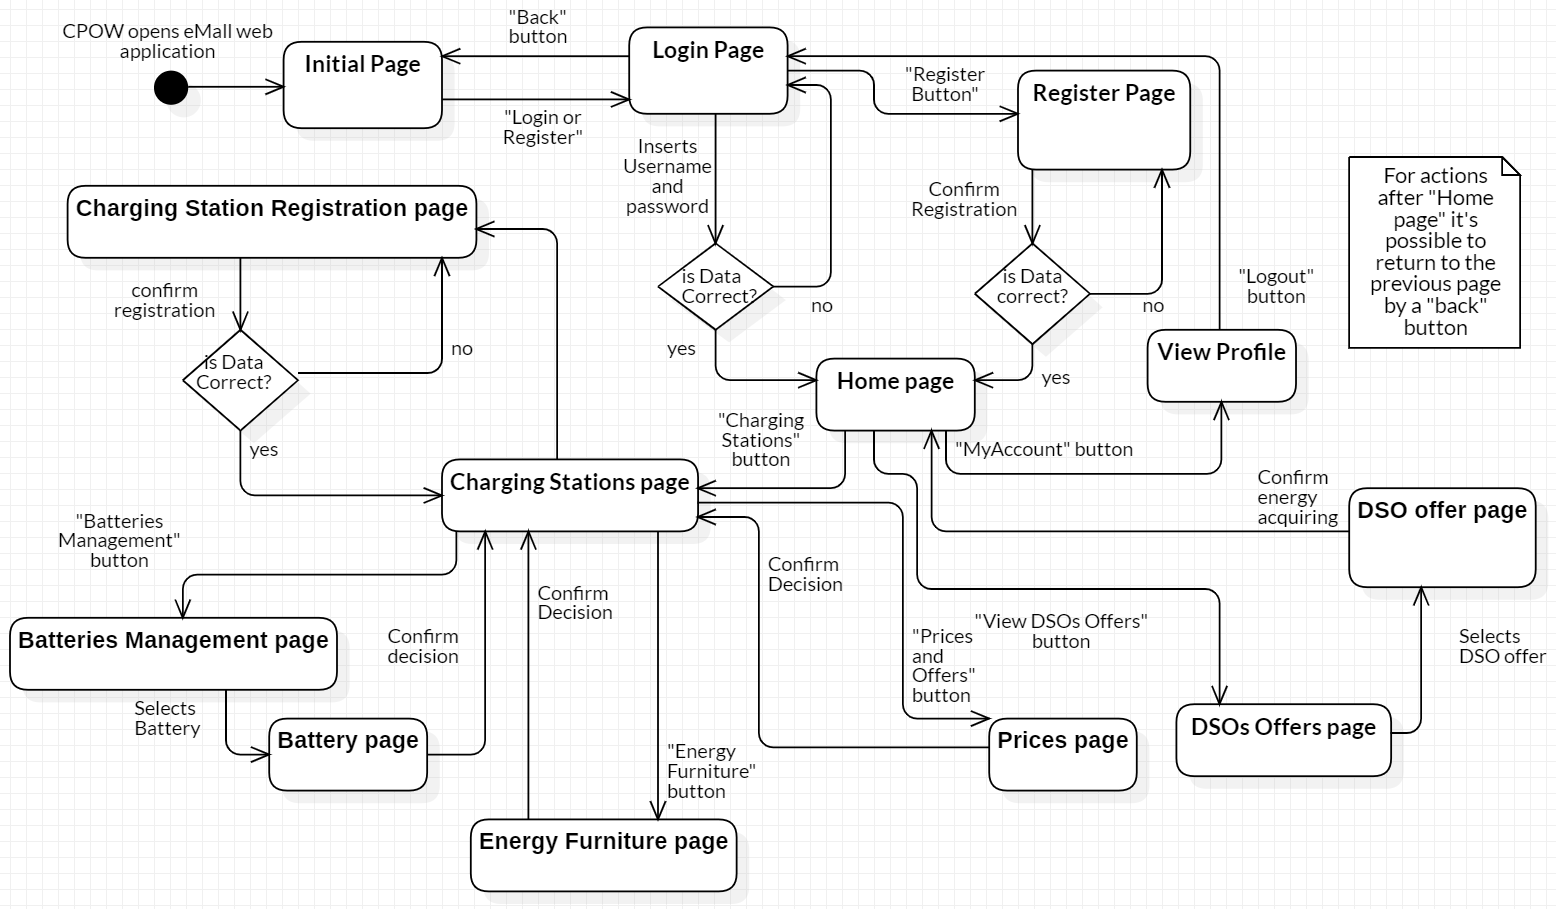
\includegraphics[angle=0, scale=0.7]{img/ACTIVITY DIAGRAM CPOW.png}
\caption{UML Activity Diagram for the CPO Worker Web App navigation}
\label{fig:SupWebApp-activity}
\end{figure}
\end{landscape}
}

\chapter{Requirements Traceability}
In this section is shown how the requirements are actually ensured and which components actually ensure them. It's worth to notice that for the sake of simplicity Mobile Application and eMSP components are considered as one because they work together doing the same activities, and the Router has been ignored  but it's always involved when dealing with a request coming from one of the clients.
Table \ref{tab:req-trace} has been added to highlight for each component what requirements it ensures.
\begin{table}[H]
  \centering
  \begin{tabular}{|c|c|}
    \cline{1-2}
   	\rule{0pt}{10pt}
   	\begin{large}
    \textbf{Component}
    \end{large}&\begin{large}
    \textbf{Requirements}
    \end{large}\\  \hline
    Mobile Application / eMSP &  R1, R2, R3, R5, R6, R7, R8, R9, R10, R11, R12, R13\\ \hline
    Web Application &  R3, R5, R15, R17, R19, R21, R24, R26, R27 \\ \hline
    Notification Manager &  R12, R13\\ \hline
    Access Manager & R3, R4, R5\\ \hline
    Bookings Manager & R9, R10, R11, R14\\ \hline
    Map Manager & R1, R2, R9 \\ \hline
    DSOs Manager &  R19\\ \hline
    Charging Station Manager & R4, R15, R17, R19, R21, R24, R26, R27 \\ \hline
    DBMS & R1, R2, R4, R6, R7, R8, R15, R26, R27 \\ \hline

  \end{tabular}
\caption{Table for mapping requirements to components} \label{tab:req-trace}
\end{table}
In the following lines is explained how the requirements are provided by the components:
\begin{itemize}
    \item{[R1]} \label{R1} The system must allow unregistered/registered users to see a map of available charging stations and their prices and offers. This requirement is provided by the Mobile Application component , the DBMS component and the Map Manager Component. The Mobile Application allows the End-User to access the charging stations map/list that is provided by the Map Manager through the DBMS and the Map APIs.
    \item{[R2]} \label{R2} The system must allow unregistered/registered users to see a list of charging stations and filter on it (e.g. offers, prices and positions). This requirement is provided as the same way as requirement R2.
    \item{[R3]} \label{R3} The system must allow unregistered users to register as end user or CPOW (if they have a badge id). The Mobile application allows the End-User to fill the registration while the Access Manager checks if the data is correct and allows to store the account information into the database communicating with the DBMS.
    \item{[R4]} \label{R4} The system must verify if the all data inserted by users are correct (e.g. personal data, vehicle and payment method information, charging station ID). This requirement is provided by the Access Manager component.
    \item{[R5]} \label{R5} The system must allow registered end users or CPOW to log in through their username and password. This requirement is provided by the Mobile Application component, the Web Application component and the Access Manager Component. The End-User/CPOW can fill the username and password through the Mobile Application/Web Application, while the Access Manager component checks if all data is correct and allows store it into the database by the DBMS.
    \item{[R6]} \label{R6} The system must allow registered end users to associate vehicles to their account and keep track of them. The Mobile Application component allows the End-User to insert all vehicle information that are stored by the DBMS component.
    \item{[R7]} \label{R7} The system must allow registered end users to associate payment methods to their account. This requirement is met in the same way as requirement R6.
    \item{[R8]} \label{R8} The system must allow registered end users to view the available time-slots for a certain type of socket of a certain charging station in a specific day. The Mobile Application component allows the end user to view the above information provided by the DBMS.
    \item{[R9]} \label{R9} The system must allow registered end users to book a charge in a specific charging station. The Mobile Application allows the user to visualize the charging stations map provided by the Map Manager and fill and confirm a charge booking through the Bookings Manager.
    \item{[R10]} \label{R10} The system must allow end users to unlock a charging socket if they have booked it and it's the correct time-slot. The Mobile Application component allows the user to visualize a personal booking page where it's possible to unlock the associated charging socket by the Bookings Manager that communicates with the related CPMS.
    \item{[R11]} \label{R11} The system must let a charge start if a vehicle is correctly connected and the charging socket is unlocked. This requirement is provided by the Bookings Manager component that directly communicates with the related CPMS.
    \item{[R12]} \label{R12} The system must show to end users the charging status (e.g. remaining time to complete charge). This requirement is met by the Mobile Application component and the Notification Manager component. The Mobile Application component provides the End-User with the information sent by the Notification Manager, which is directly connected to the related CPMS.
    \item{[R13]} \label{R13} The system must notify the end-user when the charge is complete. This requirement is provided in the same way as requirement 12
    \item{[R14]} \label{R14} When a charging process is correctly finished the system must charge on the end user selected payment system the correct import. This requirement is provided by the Bookings Manager component that is directly connected with the right Payment API.
    \item{[R15]} \label{R15} The system must allow CPOW to register a new charging station through its physical id. The Web application allows a CPOW to insert all information related to the registration which are checked and than saved by the Charging Station Manager that communicates with the DBMS.
    \item{[R16]} \label{R16} The system must be able to dynamically select if using batteries, directly the network or a mix of the two for each charging station.*
    \item{[R17]} \label{R17} The system must allow CPOWs to manually select if using batteries, directly the network or a mix of the two for each charging station associated to them. **
    \item{[R18]} \label{R18} The system must be able to dynamically select which DSO use to provide energy to a specific charging station.*
    \item{[R19]} \label{R19} The system must allow CPOWs to manually select which DSO use to provide energy to a specific charging station associated to them. This requirement is provided by the Web Application component and the DSO Manager component. The Web Application component allows the CPOW to select as input a DSO furniture and then the DSO Manager will communicate with the right DSO in order to execute the decision.
    \item{[R20]} \label{R20} The system must be able to dynamically decides if a certain energy furniture is destinated to a battery or directly to sockets of charging stations.*
    \item{[R21]} \label{R21} The system must allow CPOWs to manually decides if a certain energy furniture is destinated to a battery or directly to sockets of charging stations associated to them. **
    \item{[R22]} \label{R22} The system must keep track of the current status of each charging process (e.g. booked, startedCharging, etc.).*
    \item{[R23]} \label{R23} The system must keep track of the structure of each charging station (e.g. number of columns, number and type of sockets).*
    \item{[R24]} \label{R24} The system must allow CPOWs to view the structure of each charging station associated to them. **
    \item{[R25]} \label{R25} The system must keep track for each charging station of all bookings related to it.*
    \item{[R26]} \label{R26} The system must allow CPOWs to view all the bookings of a certain charging station associated to them and their status. **
    \item{[R27]} \label{R27} The system must allow CPOWs to set prices and special offers for a certain charging station associated to him. **
\end{itemize}
* R16, R18, R20, R22, R23, R25 requirements refers to the functions done automatically by the CPMS.\newline
** These requirement are provided by the Web Application component and the Charging Station Component. The Web Application component allows the CPOW to input the different decisions, while the Charging Station component executes them by communicating directly with the relevant CPMS. In the case of requirements 26 and 27, the DBMS is used to store the input information.

\chapter{Implementation, integration and test plan}
\section{Implementation and unit testing}
The implementation and test plan is defined starting from the general component diagram in Figure \ref{fig:general-component-diagram} and considering the level of importance of every component. All modules need to be tested individually using the white testing technique. Note that the external components (DSOAPI, MapsAPI, PaymentAPI , MotorizationAPI and CMPSAPI) are considered
to be available from the beginning. The system is to be developed according to the following five subparts :
\begin{enumerate}
    \item \textbf{Data}\newline
    This subpart consists of the database and the DBMS that handles it. This subpart is the most important to implement since is the core of the system.
    \item \textbf{CPO Managers*}\newline
    This subpart consists of the components that relays on the CPO Worker experience ( DSOs and Charging Station Manager ). Charging Station Manager component will be implemented as first. In order to do the testing operation both components will need a stub of the DBMS.
    \item \textbf{End-User Managers}*\newline
    This subpart consists of the components that relays on the End-User experience ( Notification, Access, Bookings and Map Manager ). The Bookings Manager component will be implemented as first. In order to do the testing operation, every component will need a stub of the DBMS, while the Notification Manager component will need also a stub of the Mobile Application component.
    \item \textbf{Router}\newline
    When all the previous components implementation is finished the Router component can be implemented. Note that the Router component need a stub of all Manager components in order to do the testing operation
    \item \textbf{Client side}\newline
    Finally the presentation layer is implemented. It is important to test the Mobile Application component on various types of mobile devices (smart-phones and tablets), with different versions of Android and iOS. The same holds for the Web Application that will need tests on various browsers (Google Chrome, Mozilla Firefox, Microsoft Edge), versions and operating systems.
\end{enumerate}
* Sub parts 2 and 3 constitute the Back-End of the system and can be implemented in parallel since they are independent of each other.
\section{Integration testing}
Following the implementation order explained above, has been chosen a \textbf{bottom-up} approach as integration testing strategy. The choice of this testing technique is clearly based on the evident hierarchical structure of the system. Note that as a consequence it will be necessary to construct drivers for each module and when a driver will be replaced by module the integration tests need to be checked again. Has been also decided to integrate elements of a \textbf{critical-module-first} approach in order to give precedence to the fundamental elements of the system in order to conduct a more important testing on them and find system-breaking bugs as early as possible. The figures below helps to practically understand the integration order of the components.\newline
\begin{enumerate}
    \item \textbf{DBMS}\par
    \begin{minipage}{\linewidth}
        \centering
        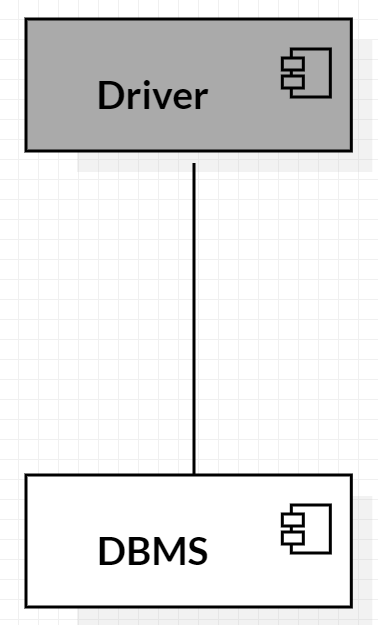
\includegraphics[scale=0.3]{img/INTEGRATION_1.png}
        \captionof{figure}{Integration DBMS}
    \end{minipage}

    \item \textbf{Back-End}\par
    \begin{minipage}{\linewidth}
        \centering
        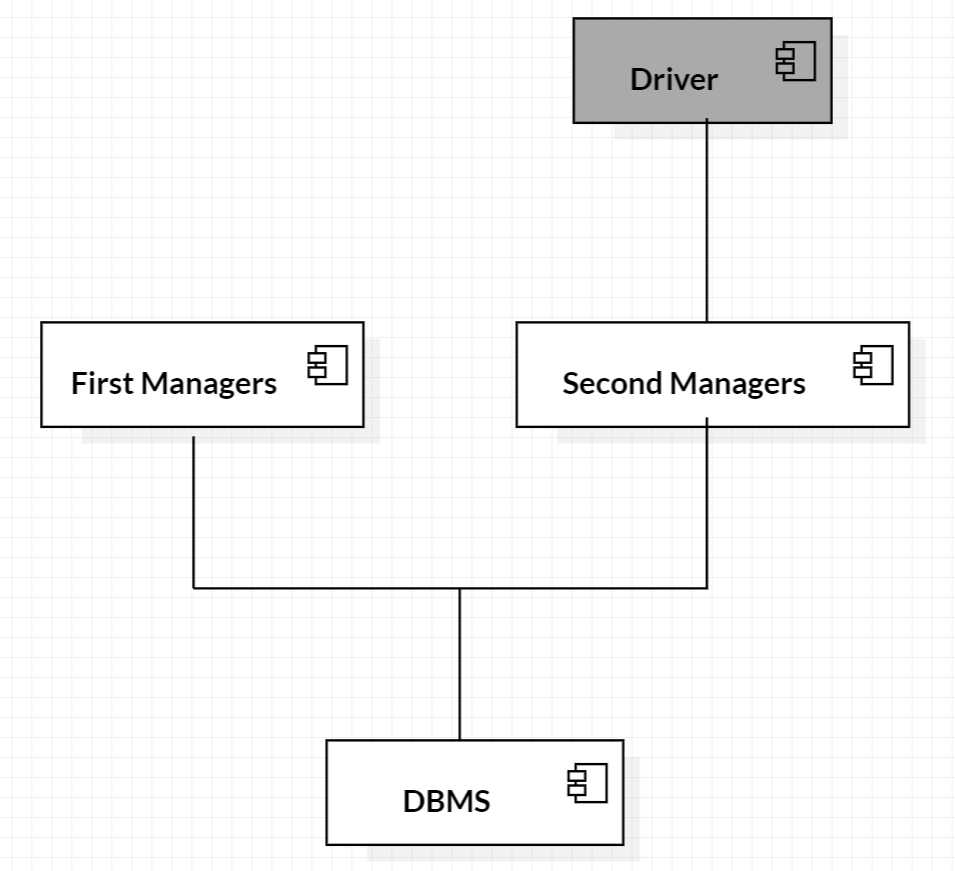
\includegraphics[scale=0.5]{img/INTEGRATION_2.png}
        \captionof{figure}{Integration Back-End}
    \end{minipage}\newline\newline

    \item \textbf{Router}\par
    \begin{minipage}{\linewidth}
        \centering
        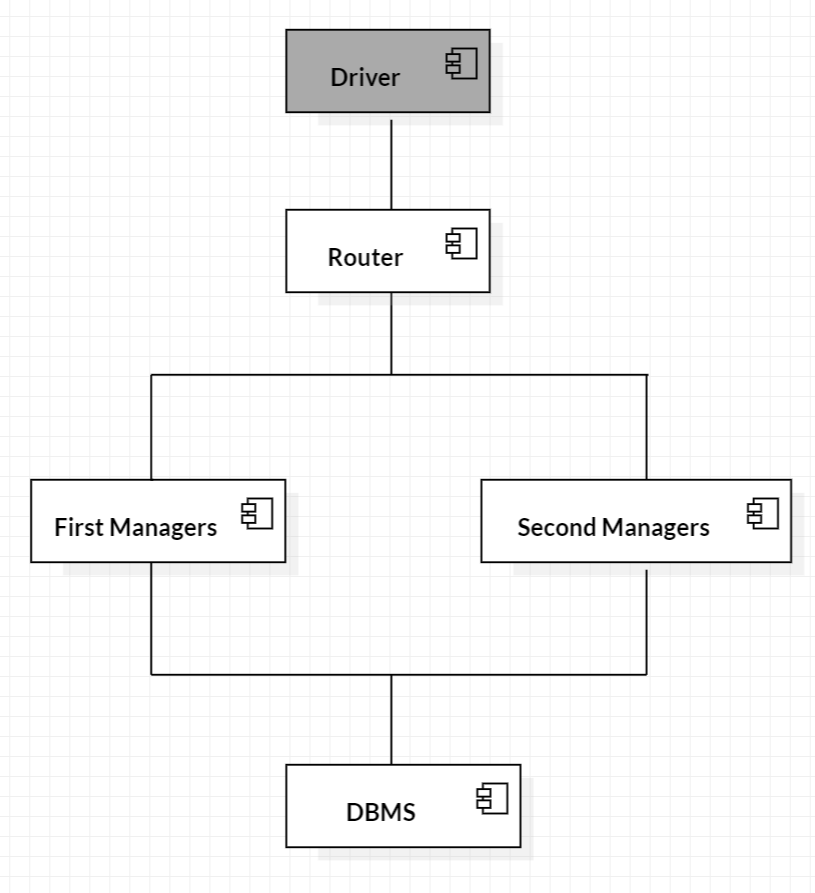
\includegraphics[scale=0.5]{img/INTEGRATION_3.png}
        \captionof{figure}{Integration Router}
    \end{minipage}

    \item \textbf{Client}\par
    \begin{minipage}{\linewidth}
        \centering
        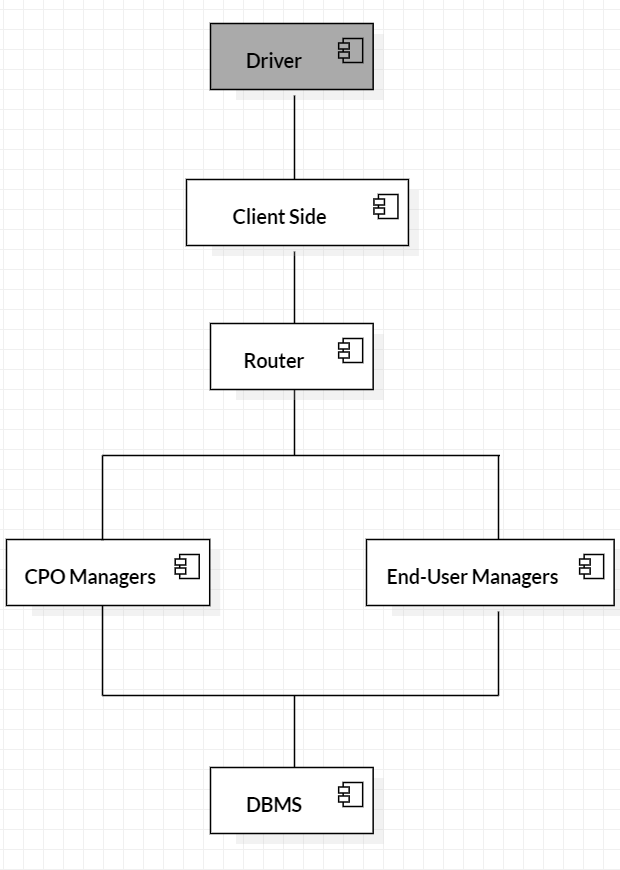
\includegraphics[scale=0.5]{img/INTEGRATION_4.png}
        \captionof{figure}{Integration Client}
    \end{minipage}
\end{enumerate}

\chapter{Effort spent}

\chapter{References}
\begin{itemize}
\item Specification Document: “Assignment RDD AY 2022-2023\_v3.pdf”
\item RASD Document: “RASD1.pdf"
\item Google Maps API: \href{https://developers.google.com/maps}{https://developers.google.com/maps}
\item Motorization API: \href{https://www.mit.gov.it/documentazione/accesso-al-sistema-informativo-motorizzazione-civile}{https://www.mit.gov.it/documentazione/accesso-al-sistema-informativo-motorizzazione-civile}
\item Payment API: \href{https://stripe.com/docs/api}{https://stripe.com/docs/api}
\end{itemize}

\end{document}


